\documentclass[aps,floatfix,superscriptaddress,twocolumn,tightenlines,amsmath,amssymb,nofootinbib,10pt,longbibliography,prl]{revtex4-2}


% ===== EXTRA PACKAGES =====
\usepackage[utf8]{inputenc}
\usepackage[T1]{fontenc}
\usepackage[mathscr]{euscript}
\usepackage{graphicx}
\usepackage[dvipsnames]{xcolor}
\usepackage{amsthm}
\usepackage{psfrag}
\usepackage{ifsym}
\usepackage{dsfont}
\usepackage{enumerate}
\usepackage{amsfonts}
\usepackage{multirow}
\usepackage{mathtools}
\usepackage{amsmath}
\usepackage{hyperref}
\hypersetup{colorlinks=true, linkcolor=red, citecolor=blue}
\usepackage[sort&compress]{natbib}
\usepackage[separate-uncertainty=true]{siunitx}
\usepackage{comment}
\usepackage[normalem]{ulem}
\usepackage[sc,osf]{mathpazo}\linespread{1.05}
\usepackage{bm}
\usepackage{bbm}
\usepackage{xr}\externaldocument[main-]{main}

\newtheorem{theorem}{Theorem}

% ===== MACROS =====
\newcommand{\bra}[1] {\langle #1 |}
\newcommand{\ket}[1] {| #1 \rangle}
\newcommand{\changed}[1]{\textcolor{red}{ #1}}
\newcommand{\todo}[1]{\textbf{\textcolor{blue}{ #1}}}
\newcommand{\new}[1]{\textcolor{brown}{ #1}}
\newcommand{\fref}[1]{Fig.~\ref{#1}}
\newcommand{\id}{\mathds{1}}


\newcommand{\sam}[1]{\textcolor{magenta}{[SB: {#1}]}}
\newcommand{\fernando}[1]{{\color{green!50!black} [JV: #1]}}
\newcommand{\mateus}[1]{{\color{blue!90!black} [GL: #1]}}
\newcommand{\victor}[1]{{\color{blue!50!blue} [VB: #1]}}


% ===== Sets ====== 
\def\ZZ{\mathbbm{Z}}
\def\RR{\mathbbm{R}}
\def\CC{\mathbbm{C}}
\def\R{\mathbbm{R}}
\def\FF{\mathbbm{F}}
\def\NN{\mathbbm{N}}
\def\EE{\mathbbm{E}}
\def\AA{\mathcal{A}}
\def\ee{\epsilon}
\def\II{\mathcal{I}}
\def\SS{\mathcal{S}}
\def\XX{\mathcal{X}}
\def\MM{\mathcal{M}}
\def\op{\mathrm{op}}
\def\aux{\textrm{aux}}
\def\1{\mathbf{1}}
\def\0{\mathbf{0}}
\def\o{\mathbb{O}}

\def\minimize{\textrm{minimize}}
\def\st{\textrm{subject to }}

\DeclareMathOperator*{\maximize}{Maximize}

\def\H{\mathcal{H}}
\def\Acal{\mathcal{A}}
\def\Fou{\mathcal{F}}
\def\Id{\mathbbm{1}}
\def\I{\mathbbm{I}}
\def\spacedot{\,\cdot\,}
\def\p{\mathbf{p}}
\def\P{\mathcal{P}}
\def\ci{\perp\!\!\!\perp}

% For the orthogonal sum
\newcommand{\operp}{\ensuremath{\text{\textcircled{$\perp$}}}}

% Operators
\DeclareMathOperator{\Sym}{Sym}
\DeclareMathOperator{\Ad}{Ad}
\DeclareMathOperator{\tr}{tr}
\DeclareMathOperator{\Tr}{Tr}
\DeclareMathOperator{\rank}{rank}
\DeclareMathOperator{\range}{range}
\DeclareMathOperator{\Span}{span}
\DeclareMathOperator{\supp}{supp}
\DeclareMathOperator{\const}{const}
\DeclareMathOperator{\Circ}{Circ}
\DeclareMathOperator{\ord}{ord}
\DeclareMathOperator{\minarg}{minarg}
\DeclareMathOperator{\sign}{sgn}

%%%%%%%%%%%%%%%%%%%

\def\b{\mathbf{b}}
\def\c{\mathbf{c}}
\def\d{\mathbf{d}}
\def\e{\mathbf{e}}
\def\t{\mathbf{t}}
\def\u{\mathbf{u}}
\def\p{\mathbf{p}}
\def\h{\mathbf{h}}
\def\q{\mathbf{q}}
\def\w{\mathbf{w}}
\def\x{\mathbf{x}}
\def\y{\mathbf{y}}
\def\z{\mathbf{z}}
\def\bxi{\bm{\xi}}
\def\bzeta{\bm{\zeta}}
\def\CC{\mathcal{C}}
\def\CD{\mathcal{D}}
\def\CP{\mathcal{P}}

\begin{document}

\title{A Hybrid Quantum–Classical Policy Network for Reinforcement-Learning Portfolio Optimization \sam{Review title}}


\author{Mateus}
\affiliation{Eldorado}

\author{Victor L. Beltran}
\affiliation{Instituto de Ciência e Tecnologia Itaú}


\author{Erhon}
\affiliation{Eldorado}

\author{Fernando}
\affiliation{Eldorado}

\author{Antonio }
\affiliation{Instituto de Ciência e Tecnologia Itaú}

\author{Samuraí Brito}
\affiliation{Instituto de Ciência e Tecnologia Itaú}


%\href{mailto:jose.scursulim@itau-unibanco.com.br}{jose.scursulim@itau-unibanco.com.br}
% \href{mailto:victor.beltran@itau-unibanco.com.br}{victor.beltran@itau-unibanco.com.br}
% \href{mailto:gabriel.langeloh@itau-unibanco.com.br}{gabriel.langeloh@itau-unibanco.com.br}
% \href{mailto:samurai.brito@itau-unibanco.com.br}{samurai.brito@itau-unibanco.com.br}


\date{\today}
\begin{abstract}

\sam{Hybrid quantum-classical neural networks are a dominant paradigm for near-term quantum machine learning, yet their impact on reinforcement learning (RL) in finance is often obscured by the high run-to-run variance of RL training. To isolate the true architectural effect, we perform a controlled ablation on an RL agent for portfolio optimization. We replace a single latent layer of a classical convocational policy benchmark with a parameterized quantum circuit and compare absent, classical, and quantum latent blocks across 20 independent runs. Using exact statevector simulation to eliminate estimation noise, we find the salient behavioral change is not a shift in mean return, but a severe contraction in policy dispersion. The coefficient of variation for the final portfolio value drops by nearly an order of magnitude compared to classical baselines. Sweeping register widths from 2 to 8 qubits produces statistically indistinguishable outcomes, indicating this stabilization stems from the bounded frequency spectrum of the variational block rather than the dimension of the Hilbert space.} %Hybrid quantum-classical neural networks are the dominant practical paradigm for applying near-term quantum devices to machine learning, yet their effect on \emph{reinforcement learning} agents in finance remains poorly characterised: most reported evidence contrasts an isolated quantum run against an isolated classical run, leaving open whether any observed difference reflects the variational block or the run-to-run variability of the training procedure itself. This paper asks a deliberately narrow question --- what changes in the behaviour of a reinforcement-learning agent for portfolio optimisation when a single latent layer of its policy network is replaced by a parameterised quantum circuit --- and answers it with a controlled ablation. Starting from the EI3 convolutional policy, we derive a scaffold architecture that can host an interchangeable latent block, and instantiate that block in three ways: absent, classical (a dense layer of eight neurons), and quantum (an eight-qubit RealAmplitudes circuit read out through $\langle Z_i \rangle$). Every remaining component --- feature extractor, decision head, reward, environment, data split and training loop --- is held fixed, and each configuration is trained \num{20} times independently. Quantum expectation values are evaluated \emph{exactly}, in statevector mode, so that the dispersion observed across runs is attributable to initialisation alone and the measured effect is the architectural effect of the variational block, free of estimation noise. Under this protocol, the salient behavioural change is not a shift in mean return but a contraction of the run-to-run dispersion of the learned policy: the coefficient of variation of the final portfolio value falls from \num{0.29} for the scaffold and \num{0.22} for its classical instantiation to approximately \num{0.03} for the quantum one, while the mean final value rises monotonically along the same ordering. A sweep over register widths of \num{2}, \num{4} and \num{8} qubits produces statistically indistinguishable outcomes, which localises the effect in the presence of the variational block rather than in the dimension of the Hilbert space it acts on --- an observation consistent with the encoding-limited frequency spectrum of a single-layer angle embedding read out through local observables.
\sam{It still needs improvement, but the previous version was too long.}
\end{abstract}
\maketitle

% =====================================================================
\section{Introduction}
\label{sec:introduction}

Quantum machine learning (QML) studies how quantum information processing can be used within learning algorithms, ranging from fault-tolerant quantum algorithms to near-term hybrid models based on parameterized quantum circuits (PQCs)~\cite{Biamonte2017Quantummachinelear,Benedetti2019Parameterizedquant,Cerezo2021Variationalquantum}. For the latter, a quantum circuit acts as a trainable function approximator embedded in an otherwise classical learning pipeline. This paradigm has motivated results on quantum feature spaces~\cite{Schuld2019QuantumMachineLear,Havlek2019Supervisedlearning}, quantum neural networks~\cite{Abbas2021Thepowerofquantumn}, and the role of data encoding in determining the functions accessible to variational models~\cite{Schuld2021Effectofdataencodi}. At the same time, the QML literature makes clear that expressive quantum models are not by themselves evidence of a practical quantum advantage: trainability, data access, fair classical baselines, and classical simulability can determine whether an apparent advantage survives careful comparison~\cite{Huang2021Powerofdatainquant,Tang2022Dequantizingalgori,McClean2018Barrenplateausinqu}.

Quantum reinforcement learning (QRL) brings these questions into the sequential decision-making setting. In variational QRL, PQCs have been used as trainable approximators for value functions and policies. Early demonstrations showed that variational circuits can be integrated into deep-RL pipelines~\cite{Chen2020VariationalQuantumCi}; subsequent work developed parametrized quantum policies~\cite{Jerbi2021ParametrizedQuantumP}, variational deep Q-learning agents~\cite{Skolik2022QuantumagentsintheGy}, and policy-gradient formulations~\cite{Sequeira2023Policygradientsusing}. These studies establish that compact quantum models can learn standard benchmark environments and, for specially constructed problem families, theoretical separations from restricted classical learners can be obtained. They do not, however, establish a generic practical advantage for variational QRL. In particular, architectural and hyperparameter choices can dominate parameter-count comparisons~\cite{Skolik2022QuantumagentsintheGy}, and recent benchmarking work has shown that conclusions of quantum outperformance can change materially when statistical uncertainty and sample complexity are treated explicitly~\cite{Meyer2025BenchmarkingQuantumR}. We therefore use ``quantum'' here to identify the parameterization of one component of the policy, not as a claim of quantum advantage.

Portfolio management is a useful testbed for this distinction. Unlike a static allocation problem, sequential portfolio optimization requires a policy to repeatedly map evolving market observations and previous allocations into new portfolio weights while accounting for the consequences of rebalancing. Deep reinforcement learning provides a natural formulation of this problem~\cite{jiang2017deepreinforcementlearningframework}, and RLPortfolio provides an open implementation of this family of environments and policy-gradient agents~\cite{RLportfolio}. Yet RL also introduces a methodological difficulty that is particularly important for hybrid quantum--classical comparisons: training outcomes can vary substantially across random initializations. A difference between one quantum run and one classical run therefore does not identify an architectural effect.

This work addresses a deliberately narrower question than whether QRL provides a quantum advantage for portfolio optimization: \emph{what changes in the behavior of an RL portfolio agent when a single latent block of its policy network is replaced by a PQC, while the remainder of the learning system is held fixed?} The distinction is important. Our experiments use exact statevector expectation values and small circuits that are classically simulable; consequently, they cannot demonstrate computational speedup, hardware advantage, or end-to-end resource advantage. Instead, the goal is to isolate the inductive effect of the variational block under controlled conditions and determine whether it changes the distribution of learned policies across independent training runs.

To make that comparison identifiable, we impose three experimental commitments. First, the quantum and classical agents differ only in the latent block and share the same feature extractor, interfaces, decision head, reward, environment, data split, and training procedure. Second, each configuration is characterized by a distribution over independent training runs rather than by a single trajectory. Third, the quantum block is evaluated using exact statevector expectation values throughout the experiments considered in this article.

Starting from the EI3 convolutional policy available in RLPortfolio~\cite{RLportfolio}, itself descended from the EIIE formulation of Jiang et al.~\cite{jiang2017deepreinforcementlearningframework}, we construct a scaffold with an interchangeable latent representation. We compare three cases: no latent layer, a classical dense latent layer, and a PQC latent layer with matched input/output width. We then vary classical width and quantum register width to examine how the observed behavior changes with the scale of the latent representation.

\sam{IMPROVE: The main contribution is therefore methodological and empirical rather than a claim of quantum superiority. We provide (i) a hybridization-ready reformulation of EI3 in which the latent-block ablation is identifiable; (ii) a repeated-run protocol that exposes the distribution of RL outcomes instead of relying on point comparisons; (iii) an empirical characterization of the effect of replacing the latent block by a variational circuit in the noiseless simulation limit; and (iv) tests of the sensitivity of this effect to register width. In the experiments reported below, the most pronounced difference is a contraction of run-to-run dispersion rather than a statistically established improvement in mean return. We interpret that observation as a property of the tested architecture and training regime, and investigate its connection to the bounded, encoding-dependent function class of the variational block rather than treating it as evidence of quantum advantage.}
% =====================================================================
\section{Background and related work}
\label{sec:background}

\subsection{Portfolio optimisation as a reinforcement-learning problem}
\label{subsec:bg-portfolio}

Portfolio optimisation is naturally sequential: an agent observes a market state, chooses a portfolio allocation, incurs transaction costs when rebalancing, and then receives a reward determined by the subsequent evolution of asset prices. Deep reinforcement learning (DRL) therefore offers a model-free way to learn dynamic allocation policies without requiring an explicit parametric model of returns. A widely used formulation is due to Jiang et al.~\cite{jiang2017deepreinforcementlearningframework}, who introduced the Ensemble of Identical Independent Evaluators (EIIE), Portfolio-Vector Memory, and a transaction-cost-aware objective for cryptocurrency portfolio management. RLPortfolio later provided an open implementation of this class of environments and policy-gradient agents, including the EI3 architecture used as the classical starting point in this work~\cite{RLportfolio}.

Recent literature has extended DRL portfolio methods to risk-aware and high-dimensional settings. For example, Jiang, Olmo and Atwi embed transaction costs and risk aversion into a TD3-based allocation framework and report strong empirical performance on large equity universes~\cite{Jiang2024DRLPortfolioSelection}. At the same time, the broader evidence is mixed. A recent taxonomy and experimental review documents substantial heterogeneity in datasets, reward definitions, evaluation protocols and baselines across the portfolio-RL literature~\cite{Rezaei2025DRLPortfolioReview}. More importantly, Kruthof and M\"uller evaluate Soft Actor-Critic across seven equity datasets and find no systematic advantage over a $1/N$ benchmark; modest transaction costs can eliminate apparent gains because of high turnover~\cite{Kruthof2025CanDRLBeat1N}. These results motivate two design choices in the present study: comparisons should be made under matched environments and costs, and conclusions should be based on distributions over independent training runs rather than isolated trajectories.

\subsection{Parameterized quantum circuits as trainable function approximators}
\label{subsec:bg-pqc}

In near-term quantum machine learning, parameterized quantum circuits (PQCs) are commonly used as differentiable function approximators embedded in hybrid quantum--classical models~\cite{Benedetti2019Parameterizedquant,Cerezo2021Variationalquantum}. A typical PQC layer comprises three elements: a data-encoding map, a trainable unitary, and a measurement rule that converts the final quantum state into classical outputs. In the present work, classical latent features are encoded through single-qubit rotations, followed by a trainable entangling circuit, and local Pauli-$Z$ expectation values are returned to the classical policy network.

The choice of data encoding is not merely an implementation detail. Schuld, Sweke and Meyer showed that variational quantum models can be written as partial Fourier series in the encoded variables, with the accessible frequencies determined by the generators used for data encoding and by how often the data are re-uploaded~\cite{Schuld2021Effectofdataencodi}. Re-uploading can systematically enrich this frequency spectrum and increase the family of functions representable by small circuits~\cite{PrezSalinas2020Datareuploadingfor}. Consequently, increasing the number of qubits does not by itself guarantee a richer dependence on each encoded variable; circuit width, data encoding, entangling structure and re-uploading play distinct roles in expressivity.

Trainability introduces a second constraint. Random or highly expressive variational circuits may exhibit barren plateaus, in which gradients concentrate near zero as the system size grows~\cite{McClean2018Barrenplateausinqu,Holmes2022ConnectingAnsatzEx}. The measurement rule also matters: for broad classes of shallow layered ans\"atze, global cost observables can induce exponentially vanishing gradients, whereas local observables can have substantially more favorable scaling under appropriate depth assumptions~\cite{Cerezo2021Costfunctiondepend}. Our use of local $\langle Z_i\rangle$ readout is therefore motivated not only by interface compatibility with a classical latent layer, but also by the better-understood trainability of local measurements. Because each Pauli expectation value lies in $[-1,1]$, the quantum block also produces a bounded latent representation; however, bounded output alone should not be interpreted as evidence of a uniquely quantum regularization effect.

\subsection{Variational quantum reinforcement learning}
\label{subsec:bg-qrl}

Quantum reinforcement learning (QRL) covers several distinct paradigms, including fault-tolerant algorithms with quantum access to the environment and near-term hybrid schemes in which PQCs replace classical function approximators inside otherwise classical RL loops~\cite{Meyer2022SurveyQuantumRL}. The latter is the regime relevant here. Chen et al. demonstrated variational quantum circuits as trainable value-function approximators for deep RL~\cite{Chen2020VariationalQuantumCi}; Jerbi et al. introduced parametrized quantum policies and proved learning advantages for specially constructed problem families while also demonstrating standard benchmark tasks~\cite{Jerbi2021ParametrizedQuantumP}; Skolik, Jerbi and Dunjko developed variational deep Q-learning agents~\cite{Skolik2022QuantumagentsintheGy}; and Sequeira, Santos and Barbosa studied policy-gradient agents with variational circuits and their trainability properties~\cite{Sequeira2023Policygradientsusing}.

These results establish feasibility, but they do not establish a generic practical advantage for PQC-based RL. Hardware imperfections can alter both training and evaluation behavior~\cite{Skolik2023Robustnessofquantumr}. More importantly, recent benchmarking work has emphasized that parameter-count comparisons are insufficient and that claims of outperformance depend critically on statistical validation, sample complexity and the strength of the classical baseline. Meyer et al. propose a statistical benchmarking methodology and show that several apparent QRL advantages become more nuanced under controlled evaluation~\cite{Meyer2025BenchmarkingQuantumR}. Kruse et al. reach a similar conclusion when comparing multiple QRL families and explicitly question whether advantage persists beyond artificial problem constructions~\cite{Kruse2025BenchmarkingQuantumRL}. This motivates treating the quantum circuit in this paper as an alternative policy parameterization whose behavioral effect must be measured, rather than as an a priori superior learner.

\subsection{Quantum reinforcement learning in finance}
\label{subsec:bg-qrl-finance}

Applications of QRL to financial decision making are only beginning to move beyond toy environments. Chen, Zhang and Chen study a hybrid PPO trading agent for sector rotation and report an important negative result: quantum-enhanced models obtain higher training rewards but underperform classical alternatives on investment metrics such as cumulative return and Sharpe ratio, illustrating the danger of reward--objective mismatch in financial RL~\cite{chen2025quantumreinforcementlearningtrading}. More recently, Gurgul, Chen and Lessmann propose variational QRL analogues of DDPG and DQN for dynamic portfolio optimisation and report risk-adjusted performance comparable to, and sometimes above, much larger classical models, while also documenting substantial end-to-end latency on cloud quantum hardware~\cite{Gurgul2026QRLPortfolio}. Both studies are valuable, but neither by itself resolves whether observed differences originate from the quantum parameterization, from model capacity, from training stochasticity, or from details of the experimental protocol.

The present work is positioned around that identification problem. Rather than asking whether a quantum agent ``wins'' a portfolio benchmark, we isolate a single latent block inside one policy architecture and keep the rest of the RL pipeline fixed. We then compare no-layer, classical-layer and quantum-layer variants over repeated independent runs and separately study register width. This design directly targets a gap highlighted by the recent QRL benchmarking literature: without matched architectures, repeated runs and statistical validation, architectural claims are difficult to distinguish from ordinary RL variance.

% =====================================================================
% GPT-REVISION: Reframed this part as experimental methodology. The previous title
% "Experimental testbed" understated that the section also defines the training,
% comparison, statistical and simulation protocols needed to interpret the results.
\section{Experimental methodology and testbed}
\label{sec:testbed}

% GPT-REVISION: Added a short roadmap so the reader knows which quantities are
% controlled before encountering implementation details.
The experiments are organised to separate four questions: (i) whether the
restructured classical scaffold changes the behavior of the EI3 baseline;
(ii) how a classical latent block behaves under the same scaffold; (iii) what is
observed when that block is replaced by a PQC with the same input and output
width; and (iv) how the quantum configuration behaves when register width is varied. The experiments are intended as controlled
comparisons within this testbed; they are not designed to establish quantum
computational advantage.

% GPT-REVISION: Dataset and environment remain first so that the experimental
% object is defined before architectures and comparisons are introduced.
\subsection{Environment, data and evaluation window}
\label{subsec:dataset}

All experiments use the RLPortfolio framework~\cite{RLportfolio}, which provides
a Gym-compatible environment for portfolio allocation together with the
policy-gradient training loop and the online-learning mechanism used during
evaluation.

The universe consists of ten equities traded on the Brazilian exchange (B3):
ABEV3, BBAS3, BBDC4, ITUB4, LREN3, PETR4, PRIO3, RENT3, VALE3 and WEGE3, with
daily closing, high and low prices retrieved from Yahoo Finance. Prices are
normalised per asset with a maximum-absolute scaler fitted exclusively on the
training window and applied unchanged to the test window; in addition, each
observation window is normalised inside the environment by its last closing
price. A single observation is therefore a tensor of shape
$3 \times 10 \times 50$ (features $\times$ assets $\times$ time window), the
window of \num{50} trading days being the history available to the agent at each
decision step.

% GPT-REVISION: "out-of-time" is retained descriptively, but the paragraph below
% explicitly limits the interpretation because the same test environment is also
% used for periodic validation and online learning.
The chronological split uses training from 2017-01-01 to 2019-12-31 and an
evaluation window from 2020-01-01 to 2020-12-31, the latter yielding \num{198} decision steps
(\num{199} portfolio-value observations including the initial state). Every
simulation starts from an initial capital of \num{100000} monetary units and
pays a proportional transaction cost of \SI{0.25}{\percent} on rebalancing. The
output layer emits eleven weights: the ten assets plus a cash position
representing the option to remain liquid and unremunerated.

% GPT-REVISION: Moved interpretive constraints next to the data definition rather
% than leaving them for Discussion. This prevents the Results from being read as
% evidence across multiple market regimes.
Two properties of this testbed delimit the scope of the empirical results.
The test window is a single year, and an atypical one, containing both a sharp
drawdown and a strong recovery; the trajectories in \ref{sec:results} therefore
describe behaviour under one realised market path, not an expectation over
market regimes. And no held-out validation partition is used: the test
environment also serves for periodic validation, and online learning is enabled
during the test episode. Both choices are inherited from the reference framework and are retained so that
all models --- baseline, classical and hybrid --- are evaluated under the same
procedure. Accordingly, the reported values should be interpreted as outcomes
for this evaluation protocol and this realised market path, rather than as an
estimate of performance across market regimes.

% GPT-REVIEW: This is deliberately left unresolved because it depends on the exact
% code path. If periodic validation influences checkpoint/model selection, calling
% the final window "out-of-sample" would be too strong.
\textcolor{red}{REVIEW: verify whether information from the 2020 environment is
used for checkpoint selection, hyperparameter decisions, early stopping, or any
other model-selection step. If so, the manuscript should avoid calling the 2020
window a strictly held-out out-of-sample test set.}

% GPT-REVISION: The protocol is separated from architectural description so the
% reader can distinguish experimental controls from model design.
\subsection{Training protocol, repetitions and summary statistics}
\label{subsec:protocol}

Because the variability of RL training across initialisations is of the same
order as the effects under study, no configuration is characterised by a single
run. Each configuration is trained \num{20} times independently, drawing from a
single pseudorandom stream seeded at the start of the batch and not
reinitialised between runs, so that each run begins from a distinct
initialisation and the batch as a whole is reproducible by re-executing the
procedure. Because architectures with different parameter counts consume the
pseudorandom stream differently, initialisations are \emph{not} paired across
models, and all comparisons between configurations are treated as independent
samples.

% GPT-REVISION: Avoided the stronger term "out-of-sample" until the role of the
% 2020 environment in validation/model selection is verified.
The quantity reported throughout is the portfolio value along the 2020
evaluation window, summarised at the last step as the \emph{final value}. Figures show
the mean trajectory with a $\pm 1$ standard deviation envelope across runs.
Dispersion is summarised through the coefficient of variation (CV), alongside
the mean and standard deviation across runs. The CV is used as a scale-normalised
description of dispersion because configurations can differ in mean final value;
it is not treated by itself as evidence of a statistically significant difference.

% GPT-REVIEW: The current manuscript describes repeated-run distributions, but the
% inferential procedure used to compare means and/or dispersions must be stated
% explicitly if statistical significance is claimed later.
\textcolor{red}{REVIEW: specify the statistical test or interval-estimation
procedure used for between-model comparisons, including whether multiple
comparisons are corrected. If no inferential test was performed, keep all claims
descriptive and avoid terms such as statistically significant.}

Two sets of training hyperparameters are used (\ref{tab:hyperparams}). The
\emph{unified protocol} applies an identical learning rate, episode count and
batch size to every architecture, and is the protocol under which all proposed
variants are evaluated; the protocol is therefore designed to reduce procedural differences between
the proposed variants. This control supports an architectural comparison, but
does not by itself establish that every observed difference is caused solely by
the latent block. The \emph{original configuration} reproduces the hyperparameters
published for the reference model~\cite{costa2023}, and is used to characterise
the baseline in its best known conditions, so that the reference implementation is also reported under its published
training conditions.

% GPT-REVISION: Removed "strongest available version", which would require a
% systematic hyperparameter search or evidence that no stronger EI3 setting exists.

\begin{table}[htbp]
  \centering
  \caption{Training hyperparameters under the two evaluated protocols.}
  \label{tab:hyperparams}
  \begin{tabular}{lcc}
    \toprule
    Hyperparameter & Unified protocol & Original configuration \\
    \midrule
    Training episodes      & 50                & 120 \\
    Batch size             & 8                 & 200 \\
    Learning rate          & $1\times10^{-5}$  & $1\times10^{-5}$ \\
    Sample bias            & 0.5               & 0.5 \\
    Action noise           & Dirichlet         & Dirichlet \\
    \quad $\epsilon$       & 0.2               & 0.2 \\
    \quad $\alpha$         & 0.01              & 0.01 \\
    Initialisation seed    & 42                & 42 \\
    Runs per configuration & 20                & 20 \\
    \bottomrule
  \end{tabular}
  \\[3pt]
\end{table}

In the sweep over the width of the quantum register, the seed is set as a
function of the width,
%
\begin{equation}
  \mathrm{seed}(Q) = 42 + Q,
  \label{eq:seed-rule}
\end{equation}
%
so that each register width is evaluated under a distinct fixed seed. We record
this explicitly because it means that, in that experiment, the effect of the
register width and the effect of the initialisation stream are not separable.
Consequently, register width and pseudorandom stream are confounded in this
sweep. The width experiment can therefore describe the observed behavior of the
tested configurations, but it cannot isolate a causal effect of register width.

% GPT-REVISION: Removed the claim that changing seeds "strengthens" a stability
% conclusion. Different seeds add a robustness check, but because width and seed
% change together they do not identify invariance to width.
\textcolor{red}{REVIEW: if the intended claim is specifically about robustness
to register width, rerun the width sweep with matched seed sets for every value
of $Q$; otherwise frame the current result as descriptive.}

% =====================================================================
% GPT-REVISION: Kept architecture in the experimental part, but changed the
% framing from an argumentative "chain that carries the paper" to a reproducible
% sequence of controlled model variants.
\section{Model variants and controlled hybridisation}
\label{sec:architectures}

This section defines the evaluated architectures and the sequence of
modifications used to introduce an interchangeable latent block. The purpose of
the sequence is to make the classical and quantum variants as comparable as the
implemented design permits, while keeping explicit the changes that are not
strictly parameter-matched.

\subsection{Baseline: EI3}
\label{subsec:arch-ei3}

The baseline is EI3 as reproduced from the reference
implementation~\cite{RLportfolio,costa2023} and shown in \ref{fig:arch-ei3}.
The observation tensor is processed by three parallel heads; their outputs are
concatenated with the previous portfolio weights and reduced by a $1\times1$
convolution directly to the eleven allocation scores, which a softmax turns into
weights.

\begin{figure}[htbp]
  \centering
  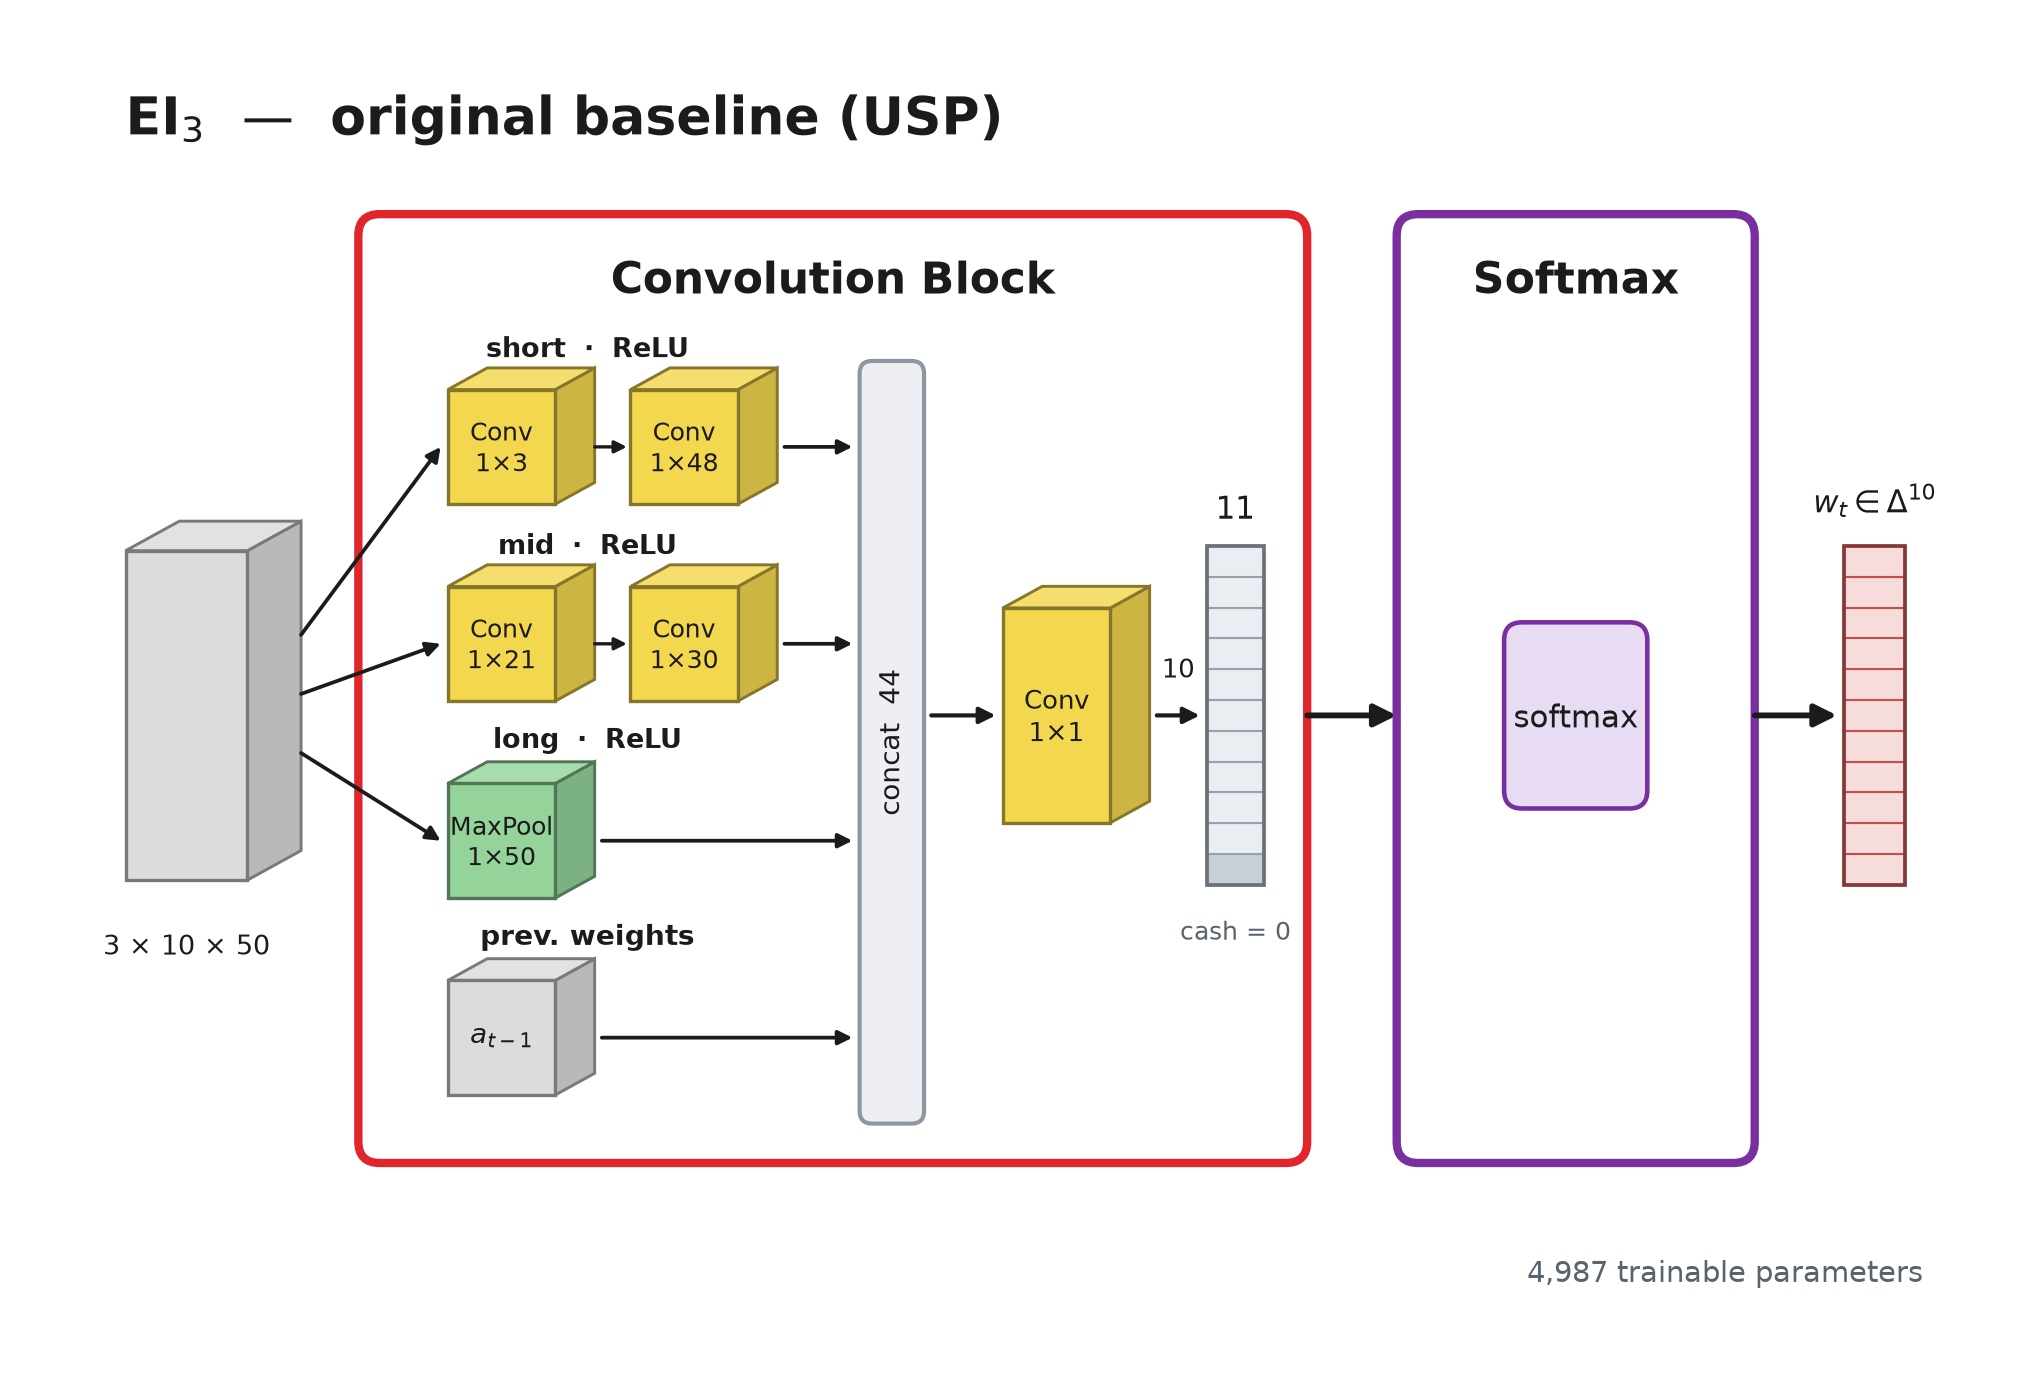
\includegraphics[width=0.85\linewidth]{figuras_finais/fig1_ei3_original.png}
  \caption{Reference EI3 architecture, as reproduced in this work. The
  observation tensor of dimensions $3 \times 10 \times 50$ (features $\times$
  assets $\times$ time window) enters a three-headed convolutional block: a
  short-term head (Conv $1\times3$ followed by Conv $1\times48$), a mid-term
  head (Conv $1\times21$ followed by Conv $1\times30$), both with ReLU
  activations, and a long-term head implemented as a MaxPool $1\times50$. The
  three outputs are concatenated with the previous portfolio weights $a_{t-1}$
  into a \num{44}-channel representation, which a final $1\times1$ convolution
  reduces to eleven scores --- the ten assets plus the cash position, held at
  zero --- normalised by a softmax into the allocation vector
  $w_t \in \Delta^{10}$. The network has \num{4987} trainable parameters. The
  proposed variants preserve this block and act only on what follows it.}
  \label{fig:arch-ei3}
\end{figure}

The property that makes EI3 a suitable point of departure is precisely the one
that makes it unsuitable as a host: the $1\times1$ convolution maps features to
allocation scores in a single step, so the network has no intermediate
representation whose width is a free parameter. There is no site at which a
block of $Q$ neurons --- or $Q$ qubits --- could be inserted without changing
the meaning of the surrounding layers.

\subsection{Design constraints imposed by a quantum latent block}
\label{subsec:design-constraints}

Creating such a site requires three design changes in the implementation used
here. They are introduced to provide a compatible interface for the latent block,
not as evidence that this restructuring is uniquely required for quantum models.

\paragraph{A latent projection with bounded angles.}
A dense projection maps the eleven convolutional channels to $Q$ values,
followed by a $\pi\tanh(\cdot)$ scaling that constrains them to $[-\pi,\pi]$.
The bound is not cosmetic. Angle encoding is $2\pi$-periodic, so unbounded
pre-activations would alias distinct market states onto the same rotation angle,
and the resulting many-to-one map would be invisible to the loss while
corrupting the representation. Restricting the encoded angles to this interval limits the range presented to
the periodic encoding.

% GPT-REVIEW: Periodicity alone does not make the full learned mapping injective,
% and the endpoints -pi and +pi represent the same rotation up to the relevant
% quantum state/global phase convention.
\textcolor{red}{REVIEW: do not claim that the $[-\pi,\pi]$ restriction makes
the encoding injective without a precise statement of the encoding map and its
domain; the current implementation primarily bounds the angles.}

\paragraph{A decision head that consumes the block output.}
Because the block emits $Q$ values in $[-1,1]$ rather than eleven allocation
scores, a small MLP head is required to map the latent code back to the
simplex. This head is identical in every variant.

\paragraph{Removal of the gated residual branch.}
An early version of the hybrid model included a residual projection from the
latent representation around the block, combined with its output through a
learnable gate. It was removed deliberately in the experimental design. With a bypass in place, the decision head can be supplied with the
pre-block representation directly, and the gate is free to attenuate the block
towards irrelevance; the network can then reach good performance while making
essentially no use of the layer under study. Any comparison between a quantum
and a classical instantiation of that layer would then be uninformative, because
neither model is required to use it. Removing the branch ensures that the decision head receives the latent-block
output without that explicit bypass, making the block harder to ignore through
this particular residual path. The cost --- a harder optimisation problem, and the
block becoming a genuine information bottleneck --- is accepted for that reason.
% GPT-REVIEW: The manuscript currently motivates residual removal conceptually,
% but no residual-vs-no-residual experiment is reported in the extracted results.
\textcolor{red}{REVIEW: if residual removal was motivated by observed training
behavior, either report the corresponding ablation or describe the removal only
as an experimental design choice. Do not claim that training becomes infeasible
without presenting the supporting experiment.}

\subsection{The scaffold: QEI3-eq NoCL}
\label{subsec:arch-nolayer}

Applying the changes above without inserting any latent block yields the
scaffold, denoted QEI3-eq NoCL and shown in \ref{fig:arch-nolayer}: the
convolutional block feeds the latent projection, the scaled latent code feeds
the MLP head directly, and the softmax produces the allocation. This variant
exists to answer a question that must be settled before any quantum claim can be
made --- whether the restructuring itself, independently of the block, accounts
for the behaviour observed later.

\begin{figure}[htbp]
  \centering
  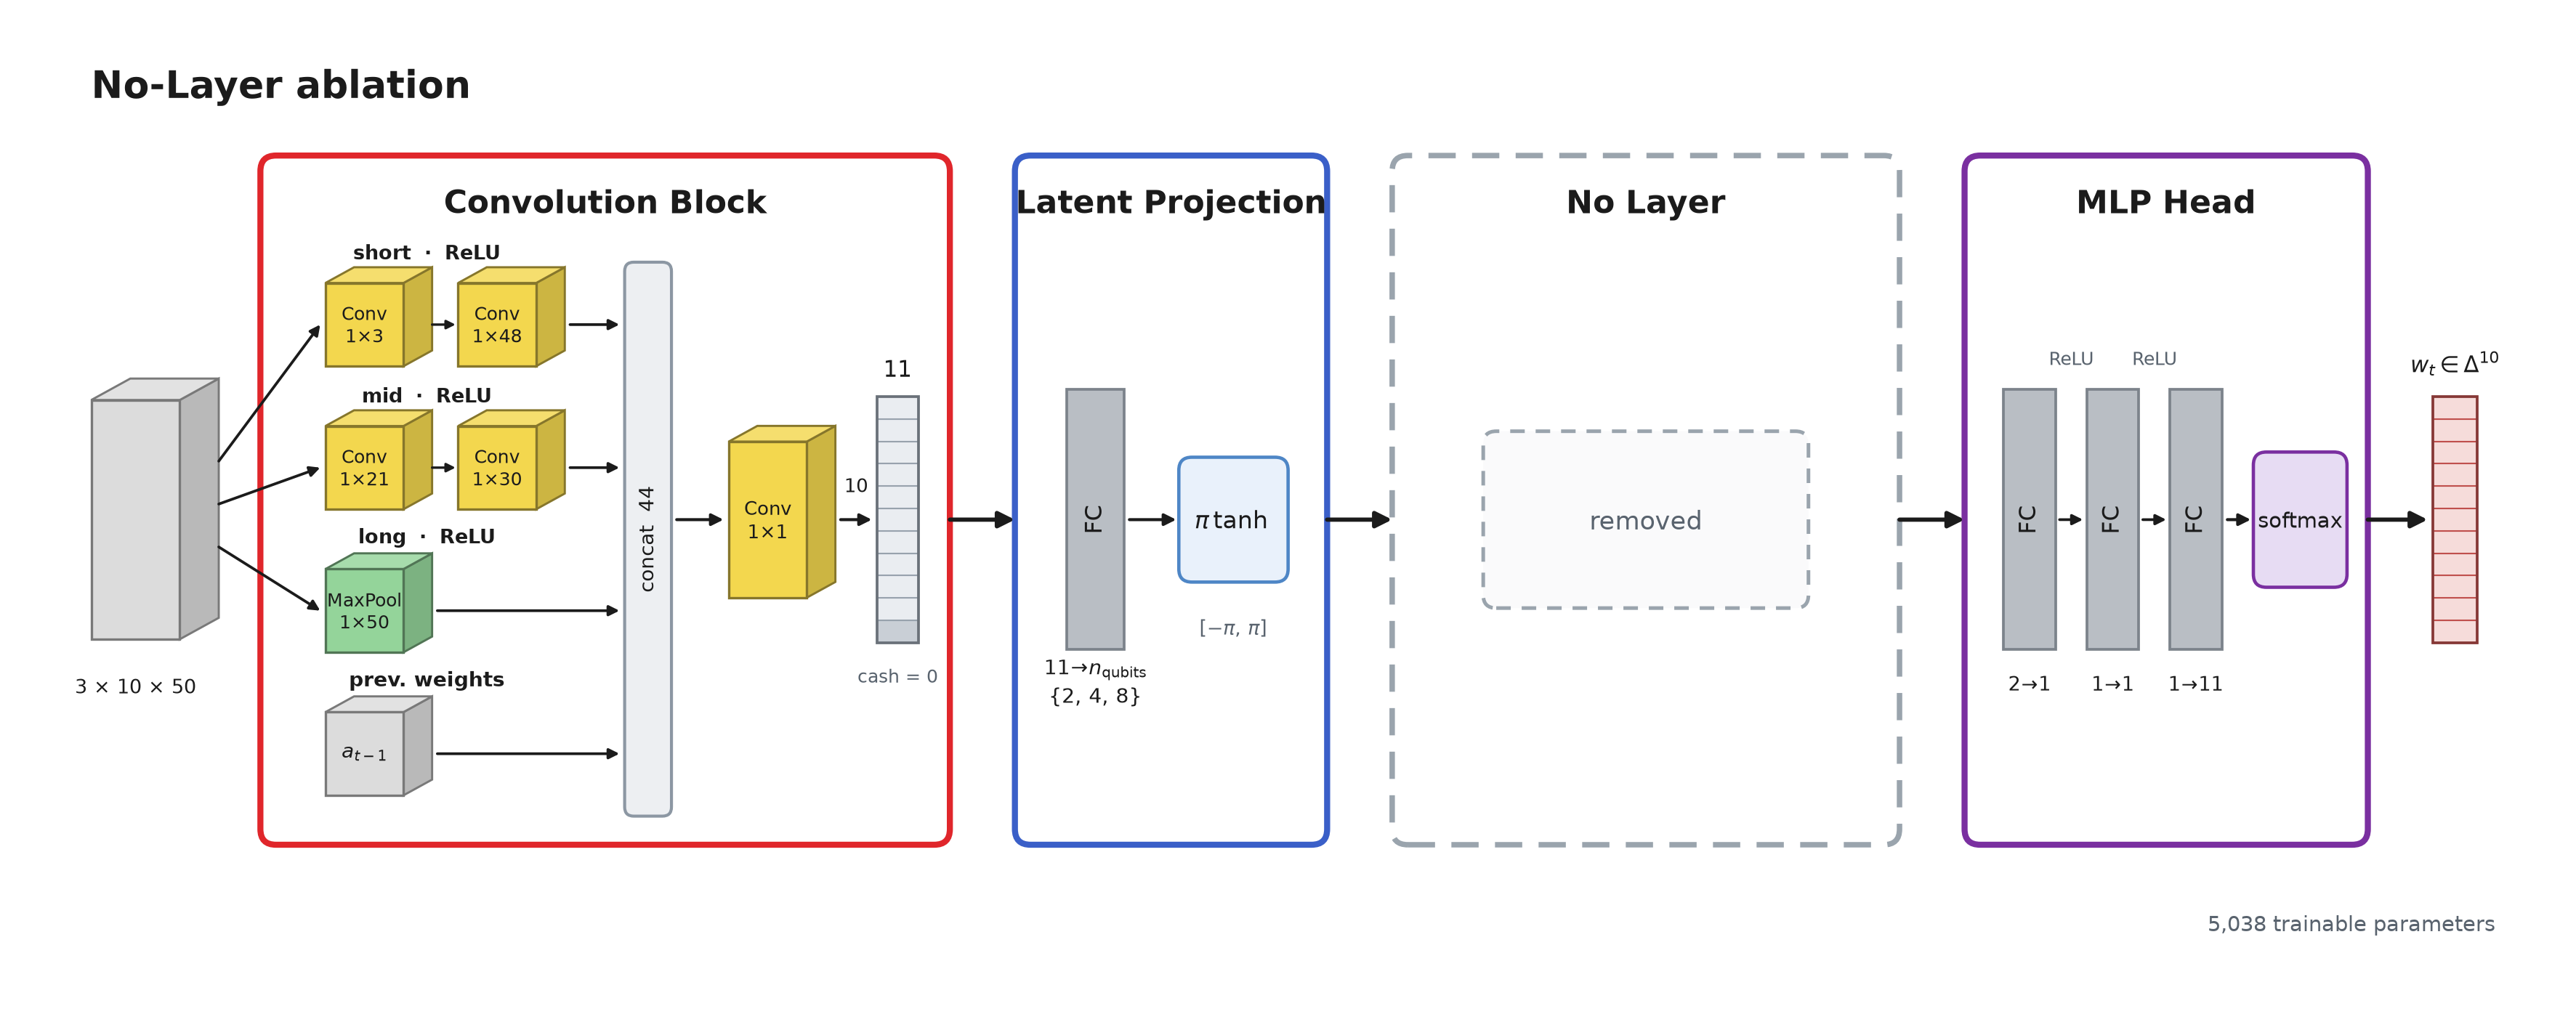
\includegraphics[width=\linewidth]{figuras_finais/fig4_nolayer.png}
  \caption{The No-Layer scaffold, QEI3-eq NoCL. The architecture is that of
  QEI3-eq (\ref{fig:arch-classical}) with the latent block removed: the latent
  projection, with its $\pi\tanh(\cdot)$ scaling, feeds the MLP head directly.
  Convolutional block, projection, decision head and softmax are unchanged, so
  the difference in behaviour between this variant and QEI3-eq is attributable
  to the latent block alone. The ablation removes six parameters,
  \num{5038} against \num{5044} for QEI3-eq in the two-wide instance drawn here,
  which keeps the total parameter counts close in this two-wide comparison.

  % GPT-REVISION: Replaced "essentially the same capacity". Similar parameter
  % count does not establish equal function-class capacity.}
  \label{fig:arch-nolayer}
\end{figure}

\subsection{Classical instantiation: QEI3-eq}
\label{subsec:arch-classical}

QEI3-eq (\ref{fig:arch-classical}) instantiates the latent block classically,
as a dense layer of width $Q$ with $\tanh$ activation. The activation is chosen
to match the range of the quantum readout: since $\langle Z_i \rangle \in
[-1,1]$ by construction, a classical surrogate with unbounded output would
differ from the quantum block in codomain as well as in parameterisation, and
the ablation would no longer isolate a single factor. At the reference width of
eight, the block contributes \num{72} trainable parameters --- a
$8 \times 8$ weight matrix and eight biases --- against roughly
$5\times10^{3}$ in the surrounding network.

\begin{figure}[htbp]
  \centering
  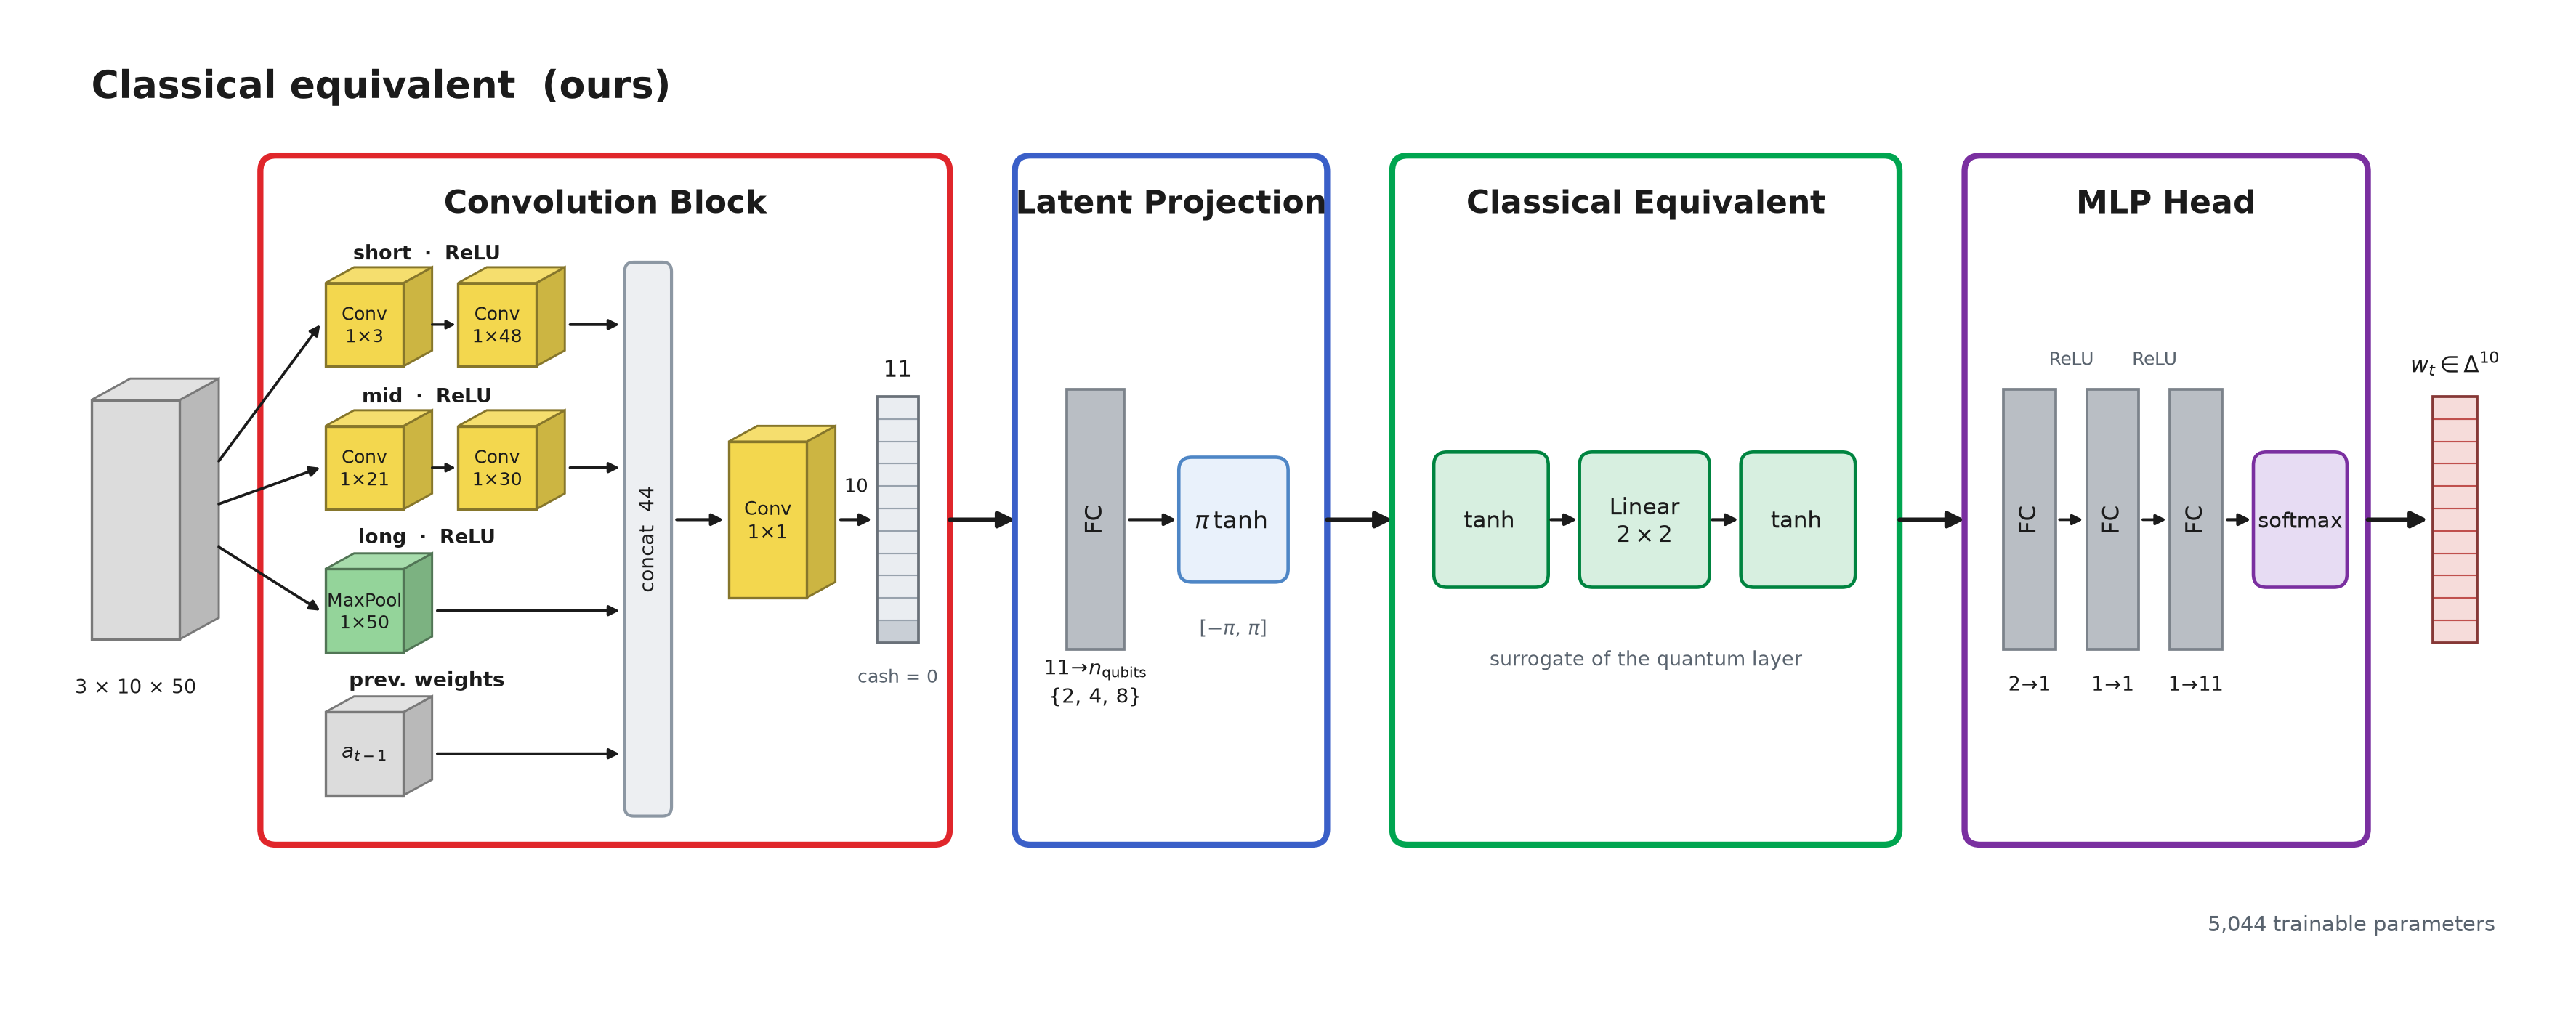
\includegraphics[width=\linewidth]{figuras_finais/fig2_classical_ours.png}
  \caption{Architecture of the proposed classical model, QEI3-eq. The
  convolutional block is inherited from EI3 (\ref{fig:arch-ei3}): the
  observation tensor of dimensions $3 \times 10 \times 50$ is processed by a
  short-term head (Conv $1\times3$ followed by Conv $1\times48$), a mid-term
  head (Conv $1\times21$ followed by Conv $1\times30$) and a long-term head
  (MaxPool $1\times50$), whose outputs are concatenated with the previous
  portfolio weights $a_{t-1}$ and reduced by a $1\times1$ convolution to eleven
  channels. A latent projection --- a fully connected layer followed by a
  $\pi\tanh(\cdot)$ scaling that constrains the values to $[-\pi,\pi]$ --- feeds
  the latent block, here a classical surrogate of the quantum layer formed by
  $\tanh$, a linear map and $\tanh$. An MLP head of three fully connected layers
  and a softmax produces the allocation vector $w_t \in \Delta^{10}$. The
  configuration drawn is the two-wide one, with projection $11\to2$ and a
  $2\times2$ linear surrogate, totalling \num{5044} trainable parameters.}
  \label{fig:arch-classical}
\end{figure}

% TODOITEM: Os diagramas das redes estão com uma diferença na dimensionalidade das camadas de transformação, isso foi gerado com base nos "qubits". Devemos re-rodar os diagramas substituindo por "n_qubits"}

\subsection{Quantum instantiation: QEI3}
\label{subsec:arch-quantum}

QEI3 (\ref{fig:arch-quantum}) replaces the same block with a variational
circuit, preserving input dimension, output dimension and position in the
network. The $Q$ scaled latent values are written into a $Q$-qubit register by
angle embedding, a RealAmplitudes ansatz with one repetition and full
entanglement is applied, and the block is read out through $\langle Z_i \rangle$
on each qubit. \ref{fig:circuit-q2,fig:circuit-q8} show the circuit at the
extremes of the sweep.

At the reference width of eight the circuit carries \num{16} trainable
parameters, against \num{72} for the classical block it replaces. This parameter-count asymmetry is part of the implemented comparison and should
be retained when interpreting any difference between the two models.

% GPT-REVISION: Parameter count is a design property, not an empirical finding,
% and it does not by itself imply parameter efficiency.

\begin{figure}[htbp]
  \centering
  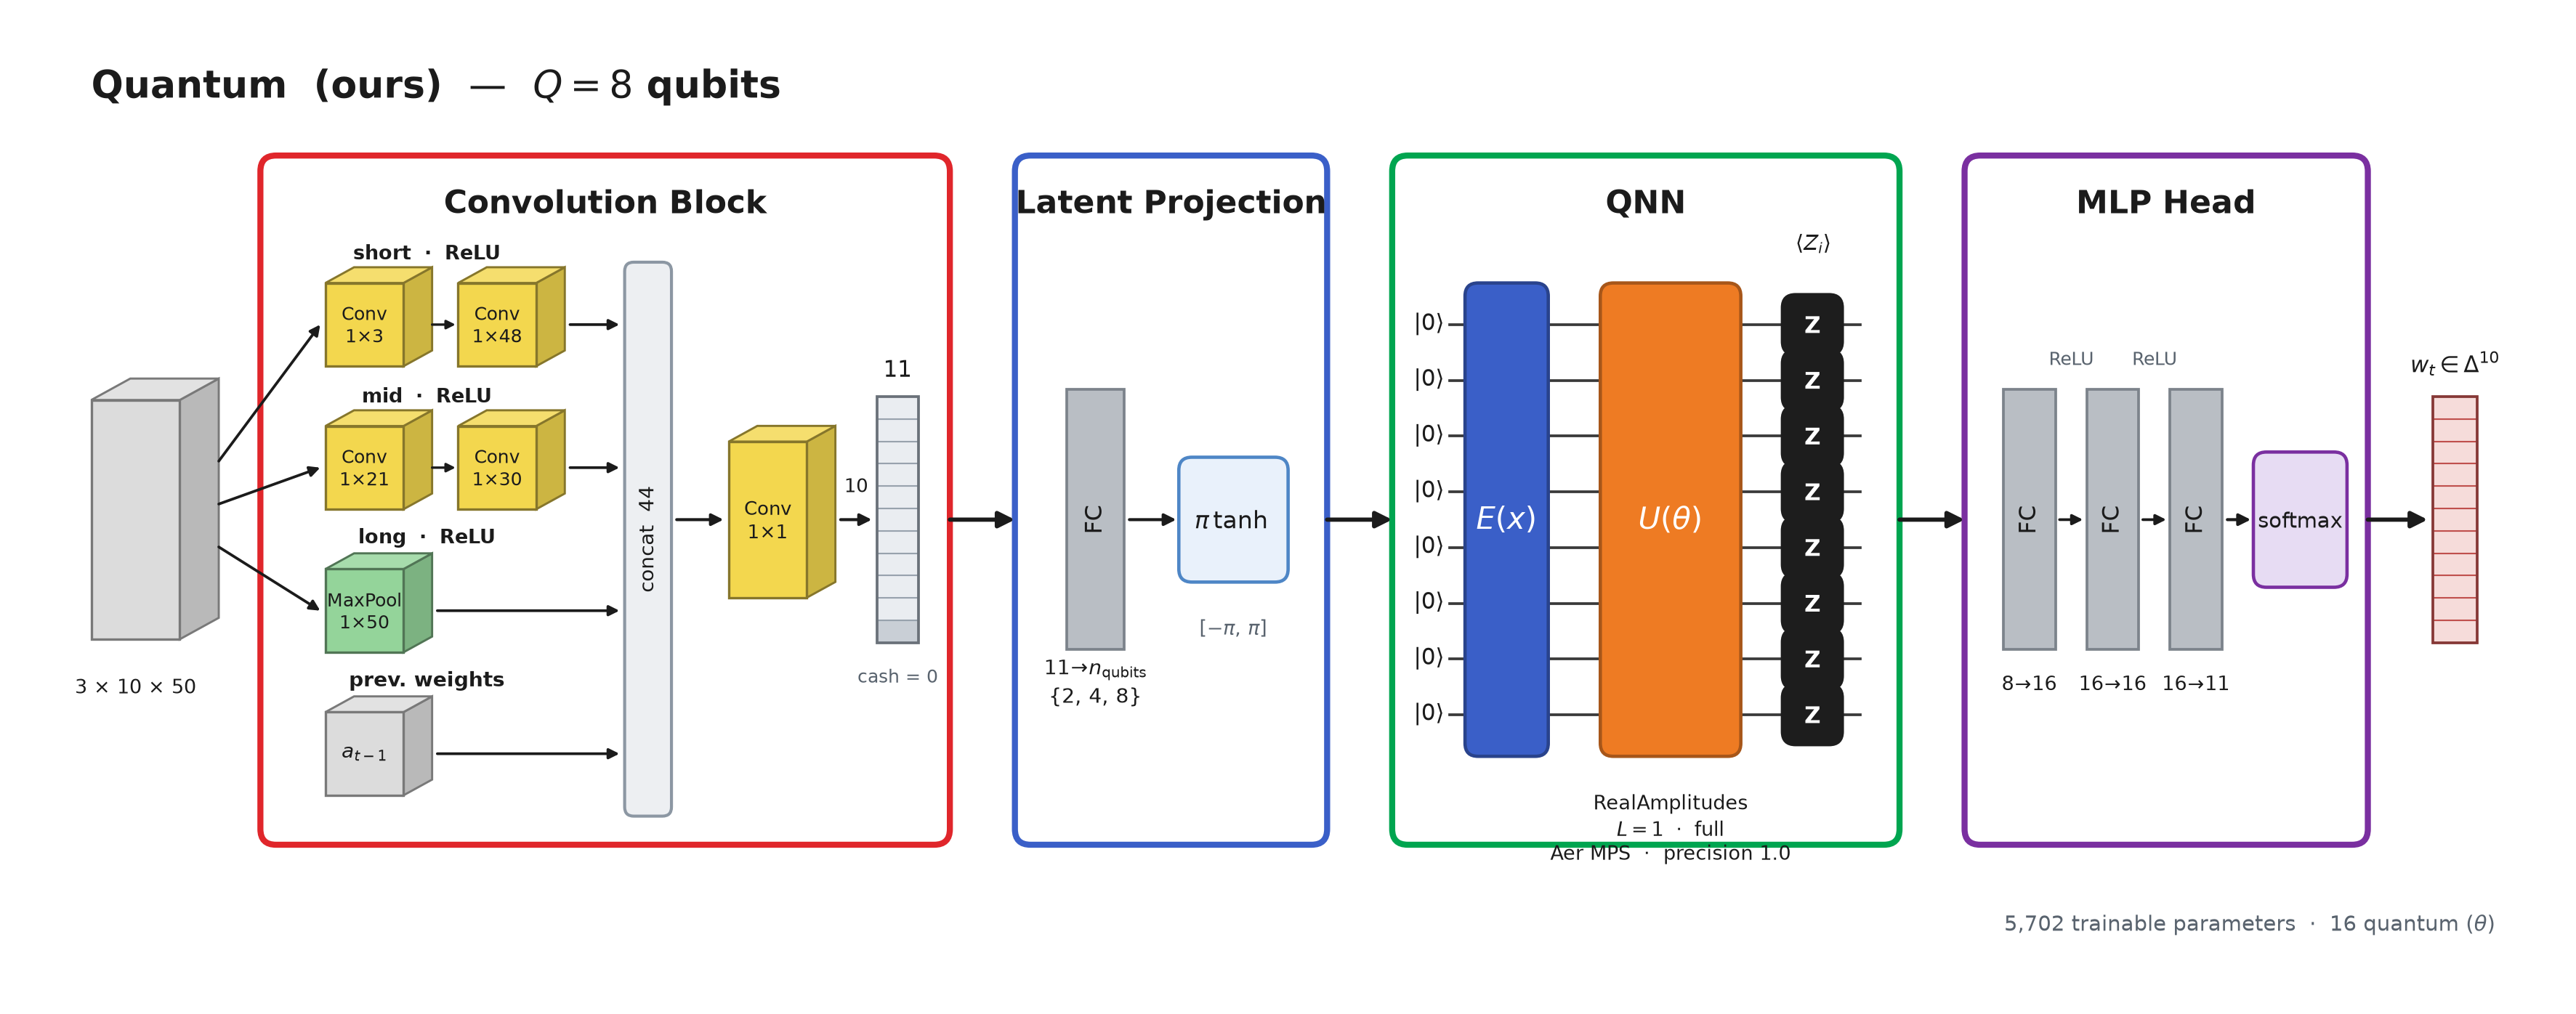
\includegraphics[width=\linewidth]{figuras_finais/fig3_quantum_ours_q8.png}
  \caption{Architecture of the proposed hybrid model, QEI3, in the
  \num{8}-qubit configuration. Convolutional block and decision head are those
  of QEI3-eq (\ref{fig:arch-classical}); the latent block alone is replaced by
  a quantum neural network. The latent projection maps the eleven convolutional
  channels to eight angles in $[-\pi,\pi]$, which the angle embedding $E(x)$
  writes into an eight-qubit register prepared in $\lvert 0 \rangle$; the
  variational unitary $U(\theta)$ is a RealAmplitudes ansatz with a single
  repetition and a full entanglement pattern, and the block is read out through
  the expectation values $\langle Z_i \rangle$ of the Pauli-$Z$ operator on each
  qubit. The eight resulting values feed an MLP head ($8\to16$, $16\to16$,
  $16\to11$) and a softmax. The model has \num{5702} trainable parameters, of
  which \num{16} are circuit parameters~$\theta$.}
  \label{fig:arch-quantum}
\end{figure}

\begin{figure}[htbp]
  \centering
  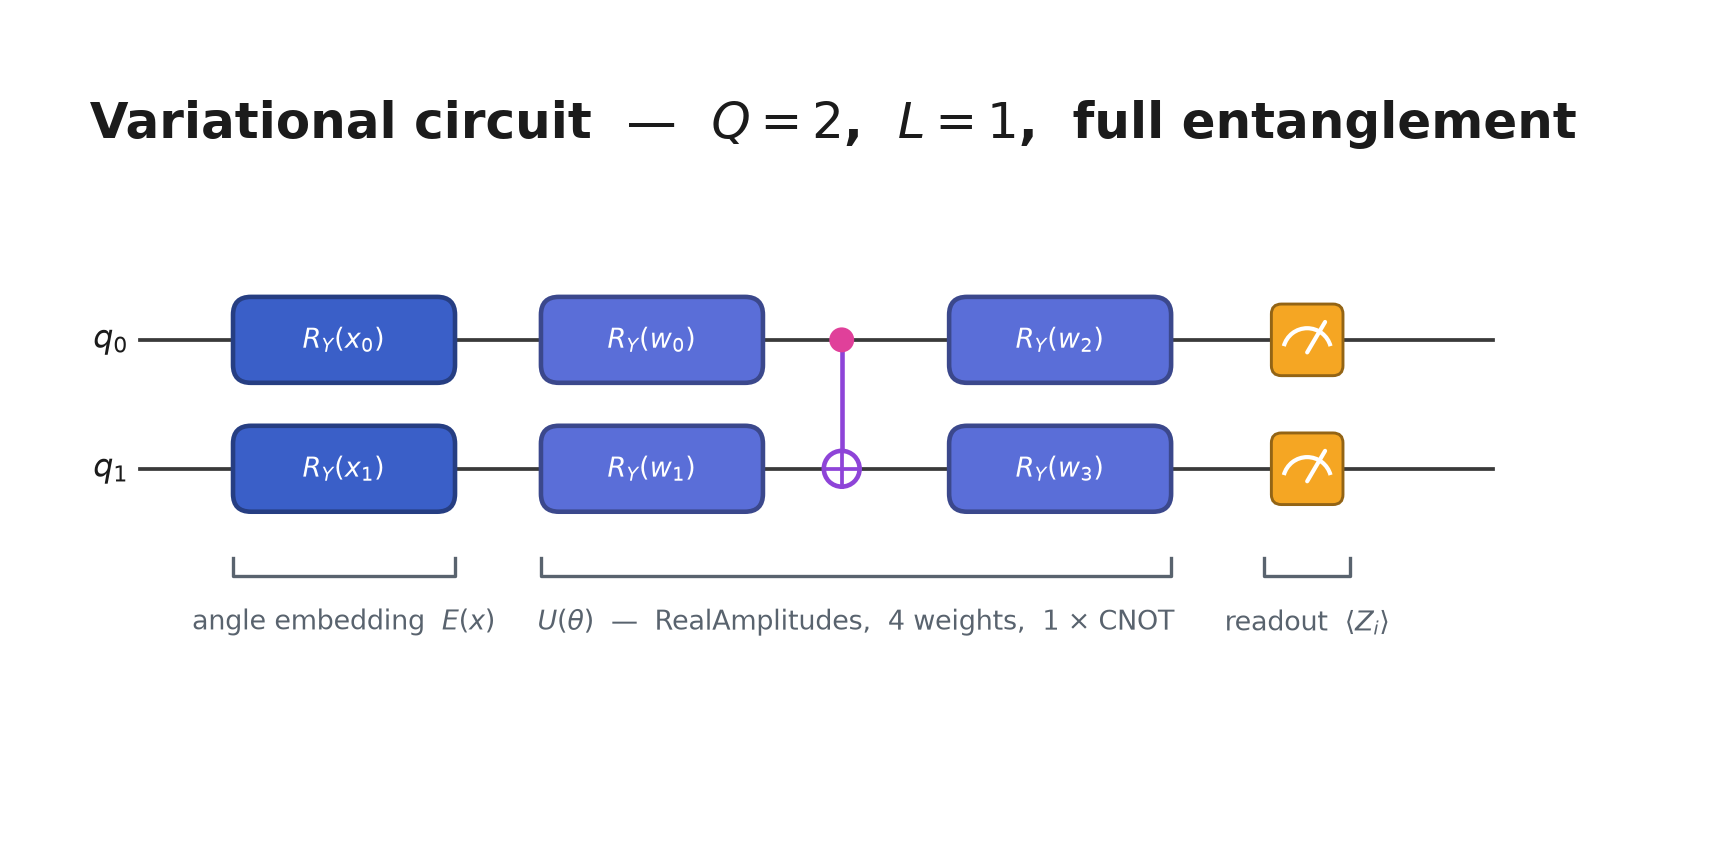
\includegraphics[width=0.9\linewidth]{figuras_finais/fig5_circuit_q2.png}
  \caption{Variational circuit of the latent block for $Q = \num{2}$ qubits,
  one repetition ($L = 1$) and full entanglement. Each qubit first receives an
  $R_Y$ rotation whose angle carries one component of the projected input
  (angle embedding $E(x)$). The RealAmplitudes ansatz $U(\theta)$ then applies a
  layer of trainable $R_Y$ rotations, a CNOT entangling the pair, and a second
  layer of trainable $R_Y$ rotations, giving four circuit weights and a single
  CNOT. The block is read out through $\langle Z_i \rangle$ on each qubit.}
  \label{fig:circuit-q2}
\end{figure}

\begin{figure}[htbp]
  \centering
  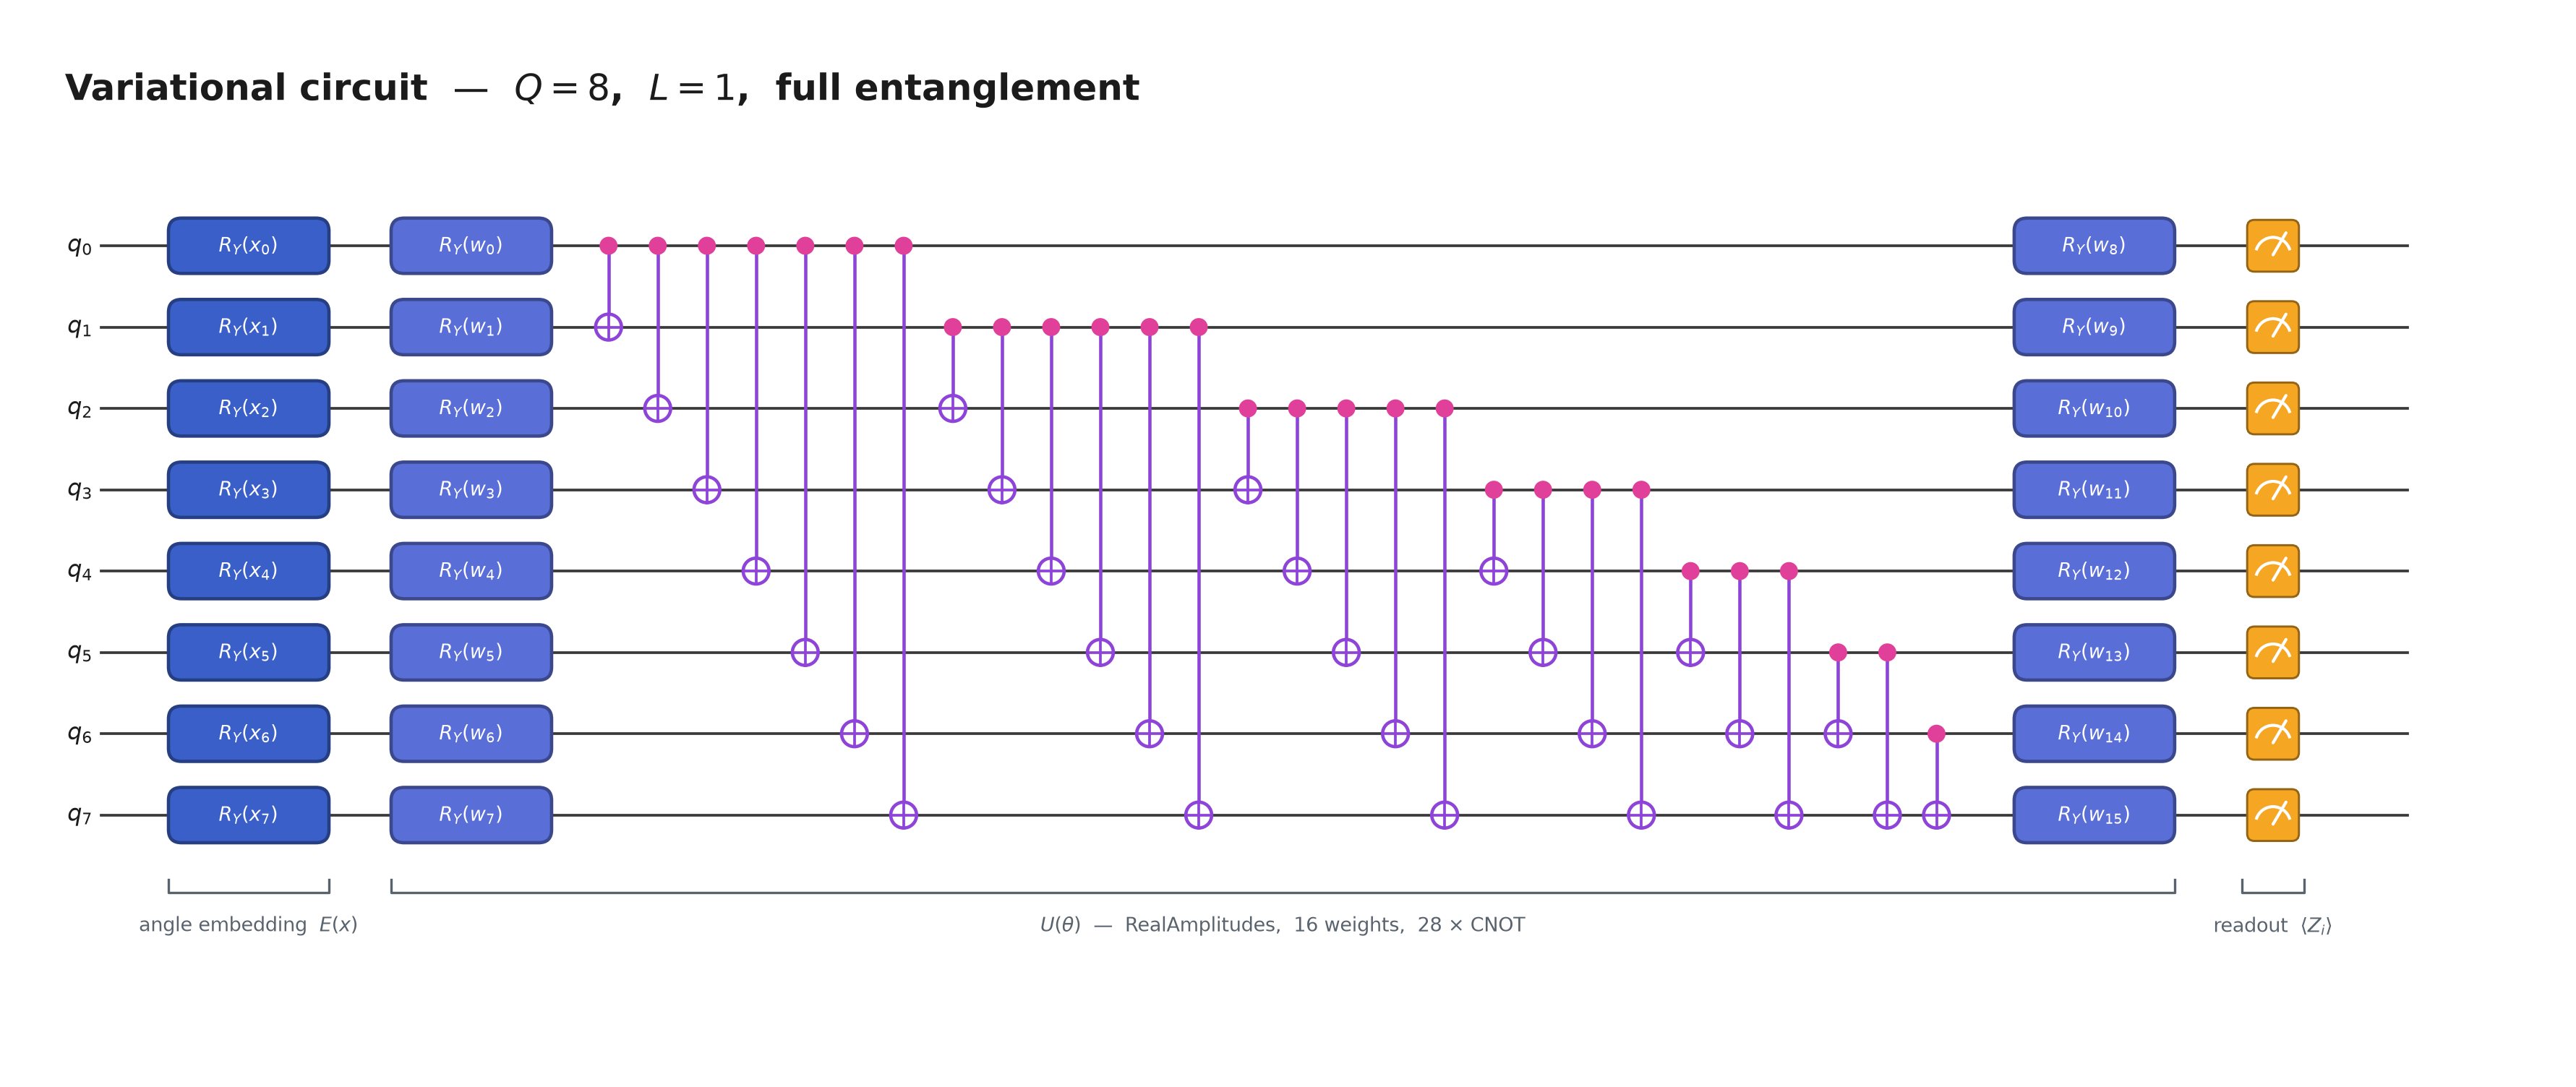
\includegraphics[width=\linewidth]{figuras_finais/fig5_circuit_q8.png}
  \caption{The same circuit at $Q = \num{8}$ qubits. The structure is unchanged
  --- angle embedding, trainable $R_Y$ layer, entanglement, second trainable
  $R_Y$ layer, and readout in $\langle Z_i \rangle$ --- but full entanglement
  now requires one CNOT for every pair of qubits: the circuit carries \num{16}
  weights and \num{28} CNOTs, against \num{4} weights and a single CNOT at two
  qubits (\ref{fig:circuit-q2}). This growth of the entangling layer, quadratic
  in the number of qubits, is what makes the simulation cost rise steeply with
  the width of the latent block, and motivates the restriction of the qubit
  sweep to \num{2}, \num{4} and \num{8} qubits. The pattern is stated explicitly
  throughout because it is not the default of the library implementation: under
  \texttt{reverse\_linear} the same specification would yield seven CNOTs at
  this width. Since $\text{reps} = 1$ places no trainable parameter between the
  two-qubit gates, the two patterns carry the same \num{16} parameters and
  differ only in the fixed entangler applied.}
  \label{fig:circuit-q8}
\end{figure}

\subsection{Implementation and simulation regime}
\label{subsec:implementation}

Circuits are built and simulated with Qiskit~\cite{qiskit2024} and integrated
with the PyTorch network through the \texttt{TorchConnector} interface, so that
the hybrid model is trained end-to-end by a single optimiser. Expectation values
are computed exactly with the \texttt{StatevectorEstimator} primitive.
% scope of this manuscript and are not discussed. Gradients
with respect to the circuit parameters are estimated by simultaneous
perturbation (\texttt{SPSAEstimatorGradient})~\cite{spall1992}, whose
perturbation directions are drawn from a dedicated pseudorandom generator seeded
independently of the training seed; circuit and network parameters are updated
jointly with AdamW.

% removed from the article at the authors' request. The manuscript now reports
% only the exact statevector simulation regime and makes no shot-related claim.
\paragraph{Simulation regime.}
All quantum experiments reported in this article use exact statevector
expectation values. This choice defines the simulation setting evaluated here;
the study does not attempt to characterize execution on quantum hardware.
The corresponding limitation is stated in \ref{sec:limitations}.

The quantum configurations evaluated are listed in
\ref{tab:quantum-configs}.

\begin{table}[htbp]
  \centering
  \caption{Quantum configurations evaluated. The ansatz is RealAmplitudes with
  $\text{reps} = 1$ and $\text{entanglement} = \texttt{full}$ in every
  configuration; gate counts are those of the logical circuit, before
  transpilation to any device connectivity (see \ref{tab:transpiled} for the
  transpiled cost). All expectation values are computed exactly; seeds follow
  \ref{eq:seed-rule}.}
  \label{tab:quantum-configs}
  \begin{tabular}{lccccc}
    \toprule
    Mode & Qubits & Circuit params. & CNOTs & Seed & Runs \\
    \midrule
    Statevector & 2 & 4  & 1  & 44 & 20 \\
    Statevector & 4 & 8  & 6  & 46 & 20 \\
    Statevector & 8 & 16 & 28 & 50 & 20 \\
    \bottomrule
  \end{tabular}
\end{table}

% =====================================================================
\section{Results}
\label{sec:results}

The results are presented in the order of the experimental chain: the baseline,
the scaffold, the classical block, the quantum block, and the matched-width
comparison. Each step isolates one factor.

\FloatBarrier
\subsection{Step 1 --- behaviour of the baseline}
\label{subsec:res-baseline}

\ref{fig:ei3-original} characterises EI3 under three training budgets before
any modification is introduced. Two observations follow.

First, the attainable level of the baseline depends on the training budget, and
the dependence is statistically detectable (Kruskal--Wallis $H(2) = 7.66$,
$p = 0.022$, $\varepsilon^2 = 0.099$), with mean final values of \num{192638},
\num{216122} and \num{224138} monetary units. The strongest configuration is
therefore the long schedule with a large batch, and it is that value ---
\num{224138} --- that any proposed variant must be compared against if the
comparison is to be fair.

Second, and more consequentially for the design of this study, the dispersion of
the baseline is substantial and grows with the budget that produces the best
mean: standard deviations of \num{31608}, \num{28132} and \num{55409}, the last
corresponding to a coefficient of variation of roughly \num{0.25}. A single
training run of this architecture is thus a weak measurement, which is the
empirical justification for the repeated-run protocol of
\ref{subsec:protocol}.

\begin{figure}[htbp]
  \centering
  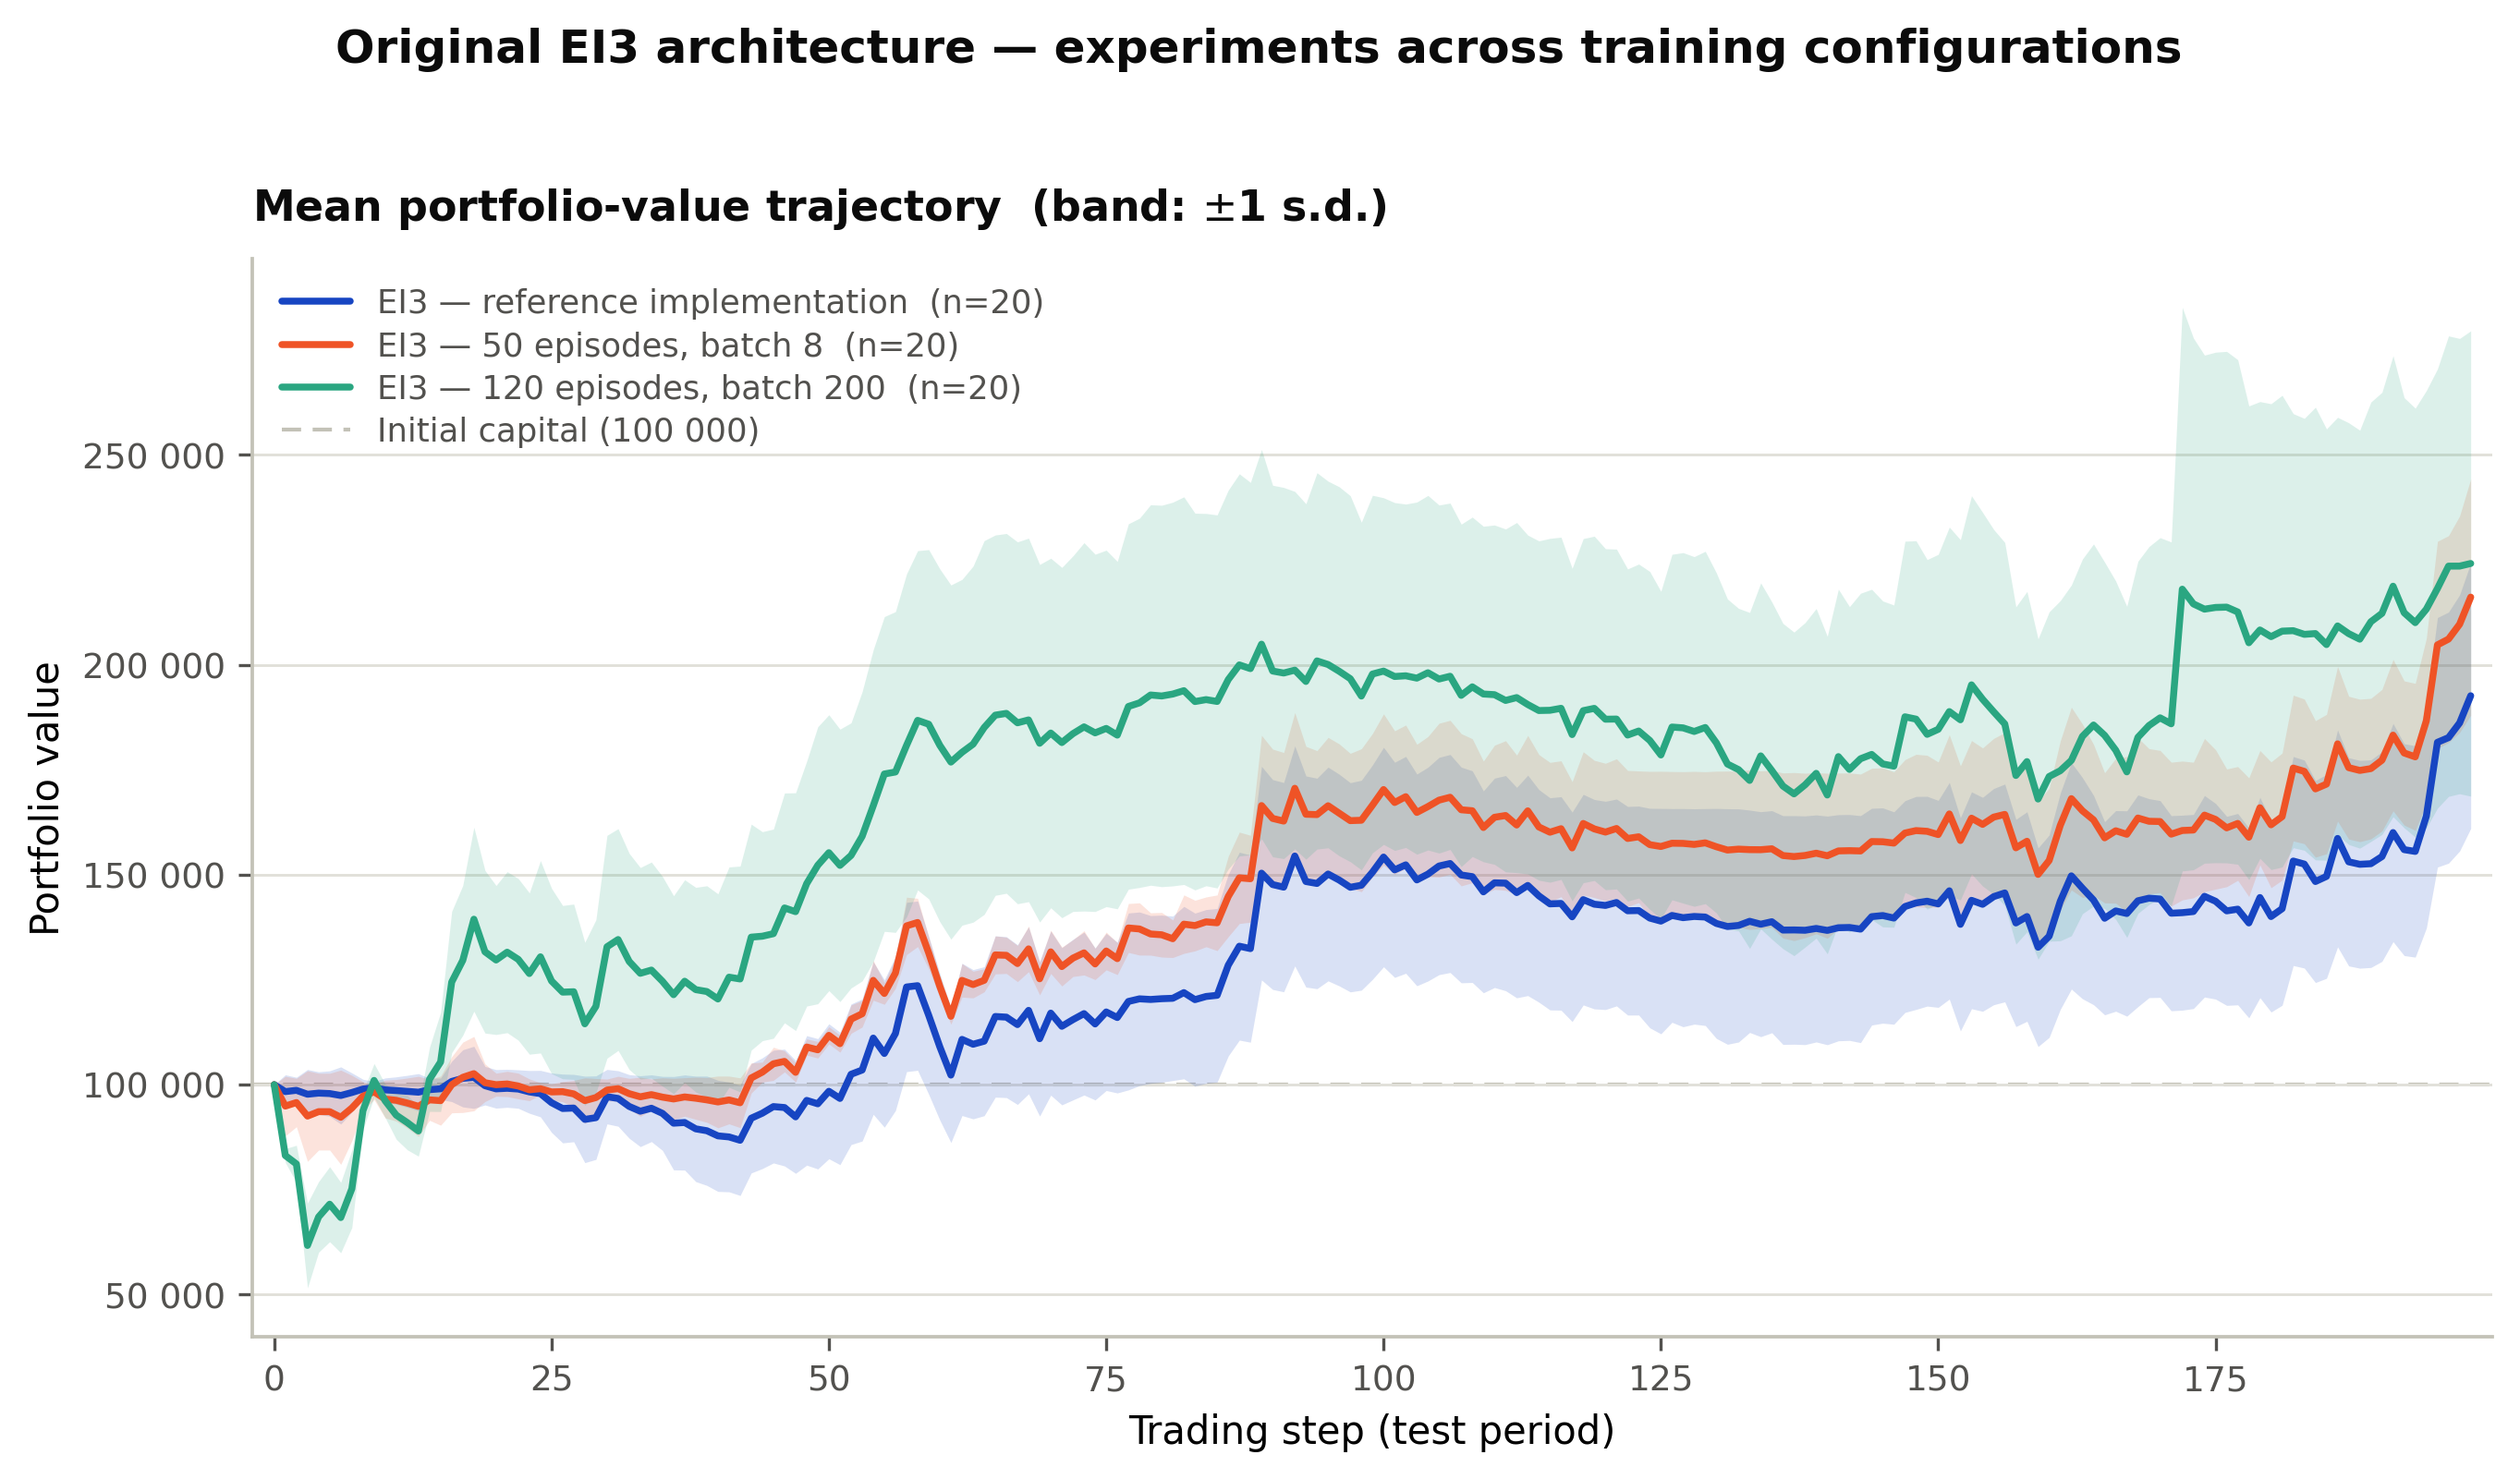
\includegraphics[width=\linewidth]{fig1_ei3_original.png}
  \caption{Original EI3 architecture under three training configurations: the
  reference implementation, a short schedule with a small batch (\num{50}
  episodes, batch \num{8}), and a long schedule with a large batch (\num{120}
  episodes, batch \num{200}). Solid lines show the mean out-of-sample portfolio
  value over the test period and shaded envelopes denote $\pm 1$ standard
  deviation across $n = 20$ independent runs per configuration; the dashed grey
  line marks the initial capital of \num{100000} monetary units. Mean final
  values are \num{192638}, \num{216122} and \num{224138} monetary units
  respectively, with standard deviations of \num{31608}, \num{28132} and
  \num{55409}. The training budget shifts the final-value distribution
  (Kruskal--Wallis $H(2) = 7.66$, $p = 0.022$, $\varepsilon^2 = 0.099$), the
  longest schedule attaining the highest mean at the cost of the largest
  dispersion across runs.}
  \label{fig:ei3-original}
\end{figure}

\FloatBarrier
\subsection{Step 2 --- does the scaffold alone account for the change?}
\label{subsec:res-scaffold}

Before attributing anything to a latent block, the restructuring itself must be
characterised. \ref{fig:no-layer} shows the twenty runs of the QEI3-eq NoCL
campaign individually, behind their mean.

The scaffold alone raises the level: its mean final value of \num{280563}
monetary units exceeds the best baseline configuration by a wide margin. Read
uncritically, this would already be a positive result. Read carefully, it is a
warning: the standard deviation across runs is \num{82410}, a coefficient of
variation of \num{0.29}, and final values span from \num{140902} to
\num{375011}. The interval covered by individual runs of the scaffold contains
the mean of every configuration reported in this paper.

The run-by-run view also shows \emph{how} the runs differ. They share the shape
of the trajectory --- the same drawdown, the same recovery, the same inflections
at the same steps --- and separate almost entirely in level. The initialisation
is not selecting between qualitatively different policies; it is scaling a
policy of largely common shape. This is the behaviour that the latent block will
be asked to control, and it is the reason why the analysis that follows treats
dispersion as a primary quantity rather than as an error bar around the mean.

\begin{figure}[htbp]
  \centering
  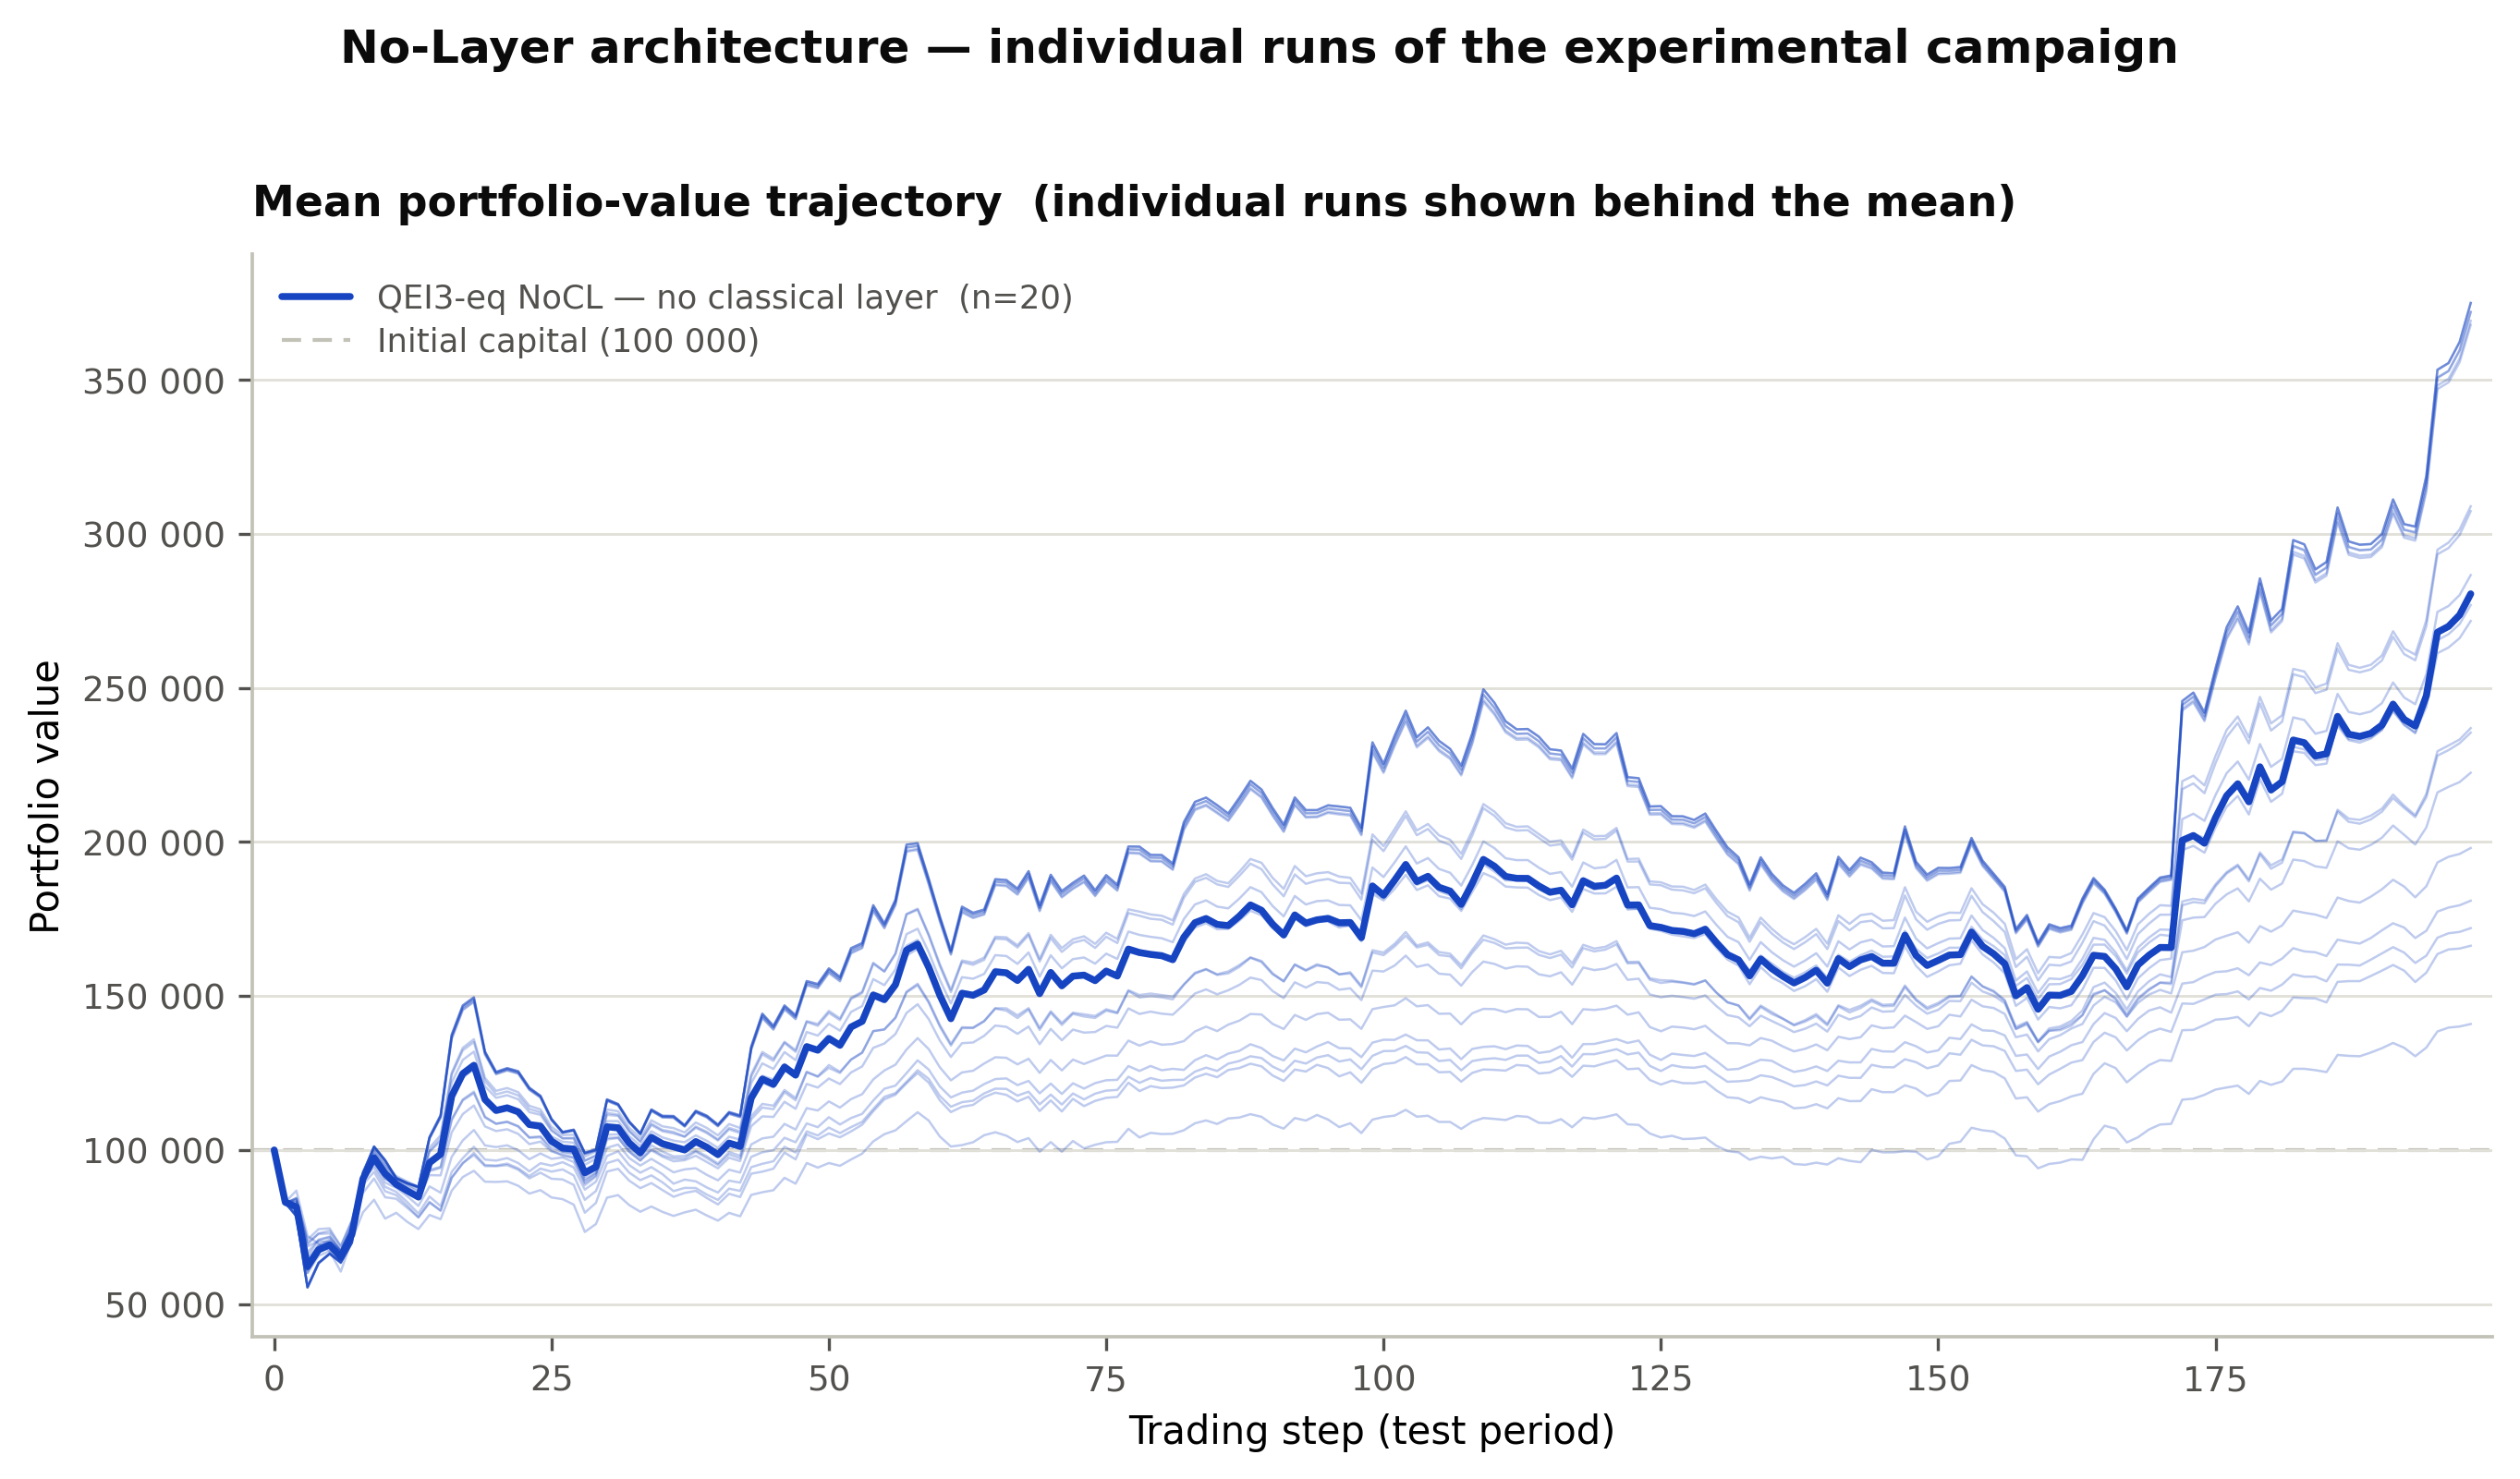
\includegraphics[width=\linewidth]{fig2_no_layer.png}
  \caption{Experimental campaign of the QEI3-eq NoCL scaffold: the \num{20}
  independent runs are drawn individually in light strokes behind their mean
  trajectory (bold), over the same out-of-sample window and initial capital as
  the remaining figures. The runs share the shape of the trajectory and separate
  mainly in level, which is what produces the wide envelope of this
  configuration in \ref{fig:layer-width}: final values range from \num{140902}
  to \num{375011} monetary units, with mean \num{280563} and standard deviation
  \num{82410}.}
  \label{fig:no-layer}
\end{figure}

\FloatBarrier
\subsection{Step 3 --- width of the classical latent block}
\label{subsec:res-classical-width}

\ref{fig:layer-width} compares the scaffold with the classical instantiation of
the block at the reference width of eight neurons, chosen to match the register
width of the quantum counterpart.

Inserting the block raises the mean final value from \num{280563} to
\num{301294} monetary units and lowers the coefficient of variation from
\num{0.29} to \num{0.22}. Both movements are in the expected direction, and
neither is decisive: at $n = 20$ per configuration the final-value distributions
are not distinguishable.

The correct reading of this result is not that the classical block does nothing.
It is that seventy-two additional parameters, placed at this position in the
network, produce an effect that this sample size cannot resolve. This
establishes the reference point for the quantum experiment: the question is no
longer whether a latent block helps in principle, but whether replacing its
parameterisation produces an effect of a magnitude that the same protocol
\emph{can} resolve.

\begin{figure}[t]
  \centering
  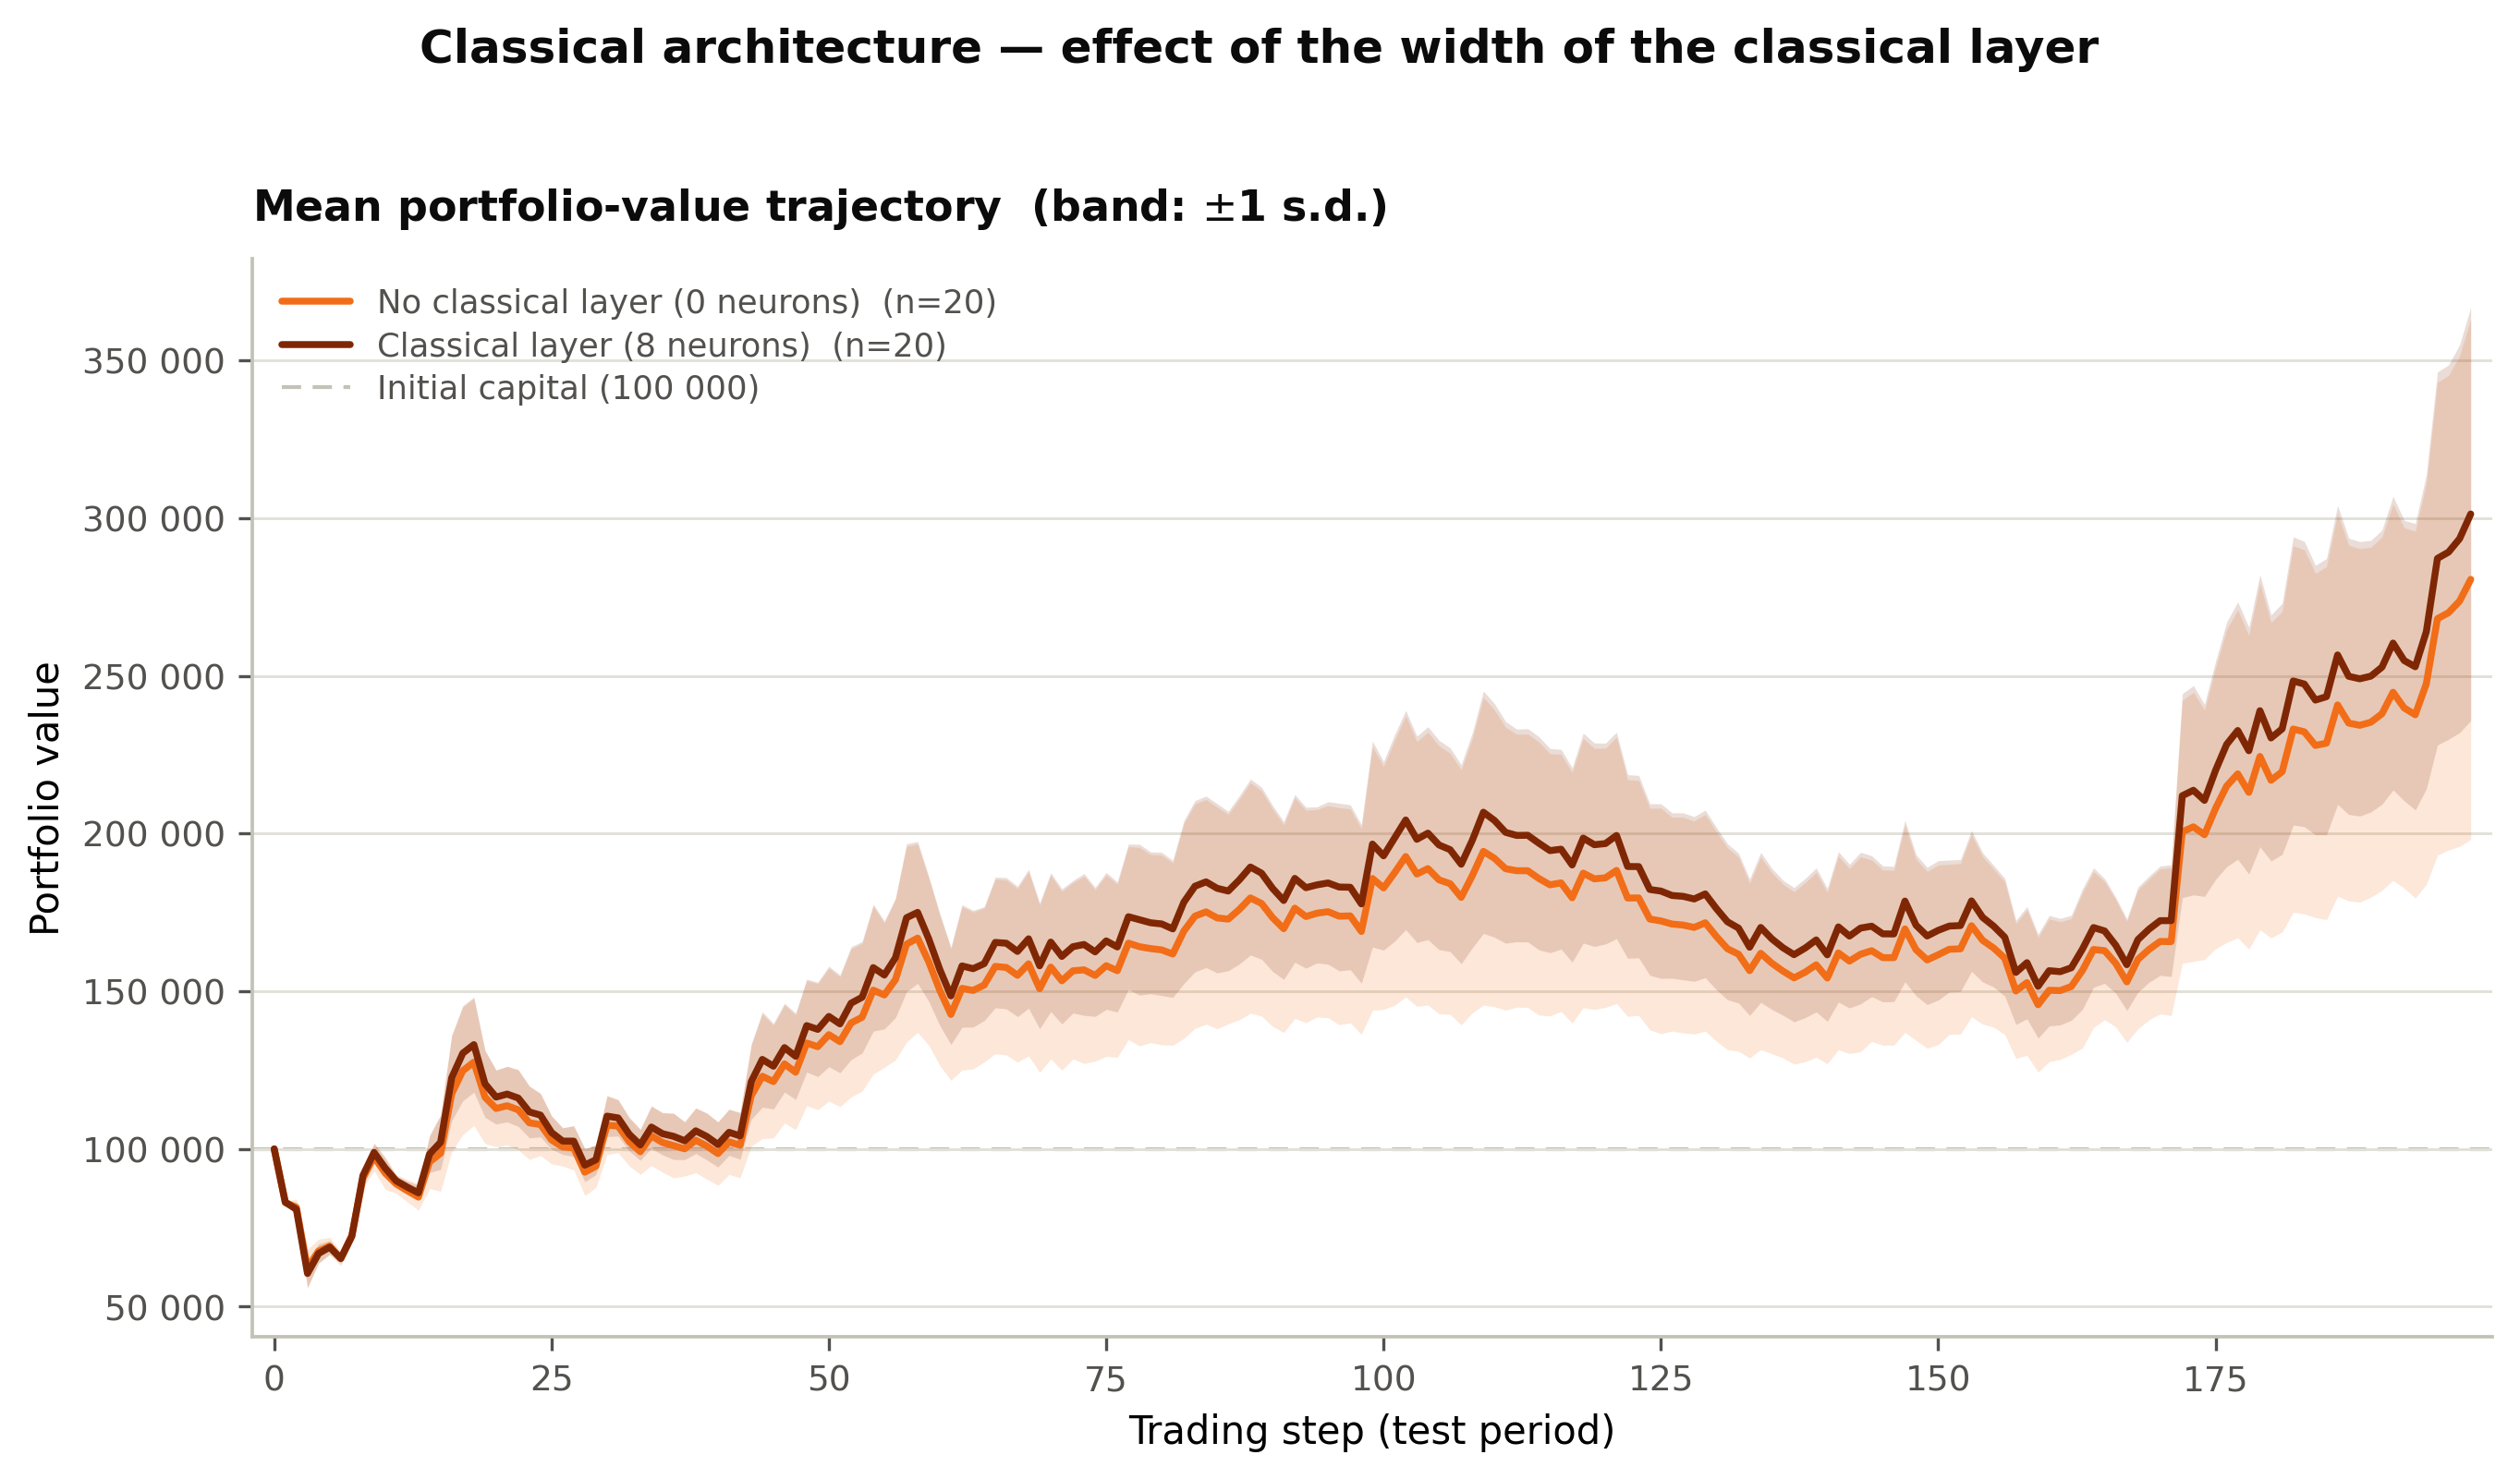
\includegraphics[width=\linewidth]{fig3_classica_neuronios.png}
  \caption{Effect of the width of the classical latent layer on the proposed
  classical architecture: QEI3-eq NoCL, without the layer (\num{0} neurons), and
  QEI3-eq with a layer of \num{8} neurons, the width that matches the number of
  qubits of the quantum counterpart. Solid lines show the mean out-of-sample
  portfolio value and shaded envelopes denote $\pm 1$ standard deviation across
  $n = 20$ independent runs per configuration. Inserting the layer raises the
  mean final value from \num{280563} to \num{301294} monetary units and lowers
  the coefficient of variation from \num{0.29} to \num{0.22}, but the
  final-value distributions are not distinguishable at the available sample size.}
  \label{fig:layer-width}
\end{figure}

\FloatBarrier
\subsection{Step 4 --- width of the quantum register under exact simulation}
\label{subsec:res-qubit-width}

\ref{fig:qubit-variation} reports the quantum instantiation at register widths
of \num{2}, \num{4} and \num{8} qubits, with expectation values computed
exactly.

Two results emerge, and they should be read together rather than in sequence.

\paragraph{The register width does not change the outcome.} Mean final values
are \num{373616}, \num{373668} and \num{369224} monetary units for two, four and
eight qubits, and the three distributions are indistinguishable
(Kruskal--Wallis $H(2) = 2.13$, $p = 0.345$, $\varepsilon^2 = 0.002$). The
effect size is essentially zero: register width explains no appreciable fraction
of the variability in final value. Since \ref{eq:seed-rule} ties each width to a
distinct seed, we do not read this as evidence that width is irrelevant in
general --- the two factors are confounded in this experiment --- but the
confound cuts in the direction that strengthens the conclusion we do draw, since
the agreement observed is agreement across three independent initialisation
streams.

\paragraph{The dispersion is an order of magnitude below anything reported so
far.} Standard deviations are \num{4327}, \num{4583} and \num{11075}, which
correspond to coefficients of variation of approximately \num{0.012},
\num{0.012} and \num{0.030}. For comparison, the same quantity was \num{0.29}
for the scaffold and \num{0.22} for its classical instantiation. Because
expectation values are exact, none of this residual spread is estimation noise:
it is initialisation variance, measured under the same protocol that produced
the much larger figures in \ref{subsec:res-scaffold,subsec:res-classical-width}.

We also note that the narrowest register is the most economical on every axis:
four circuit parameters and one CNOT against sixteen and twenty-eight at eight
qubits, with a simulation cost that grows exponentially in the register width
and a two-qubit-gate count that grows quadratically. Under the evidence
available, the cost-benefit optimum in this regime is the \emph{narrow}
register, and the eight-qubit configuration is retained in the head-to-head
comparison of \ref{subsec:res-headtohead} only because it is the width at which
the classical block was matched, not because it was measured to be better.

\begin{figure}[htbp]
  \centering
  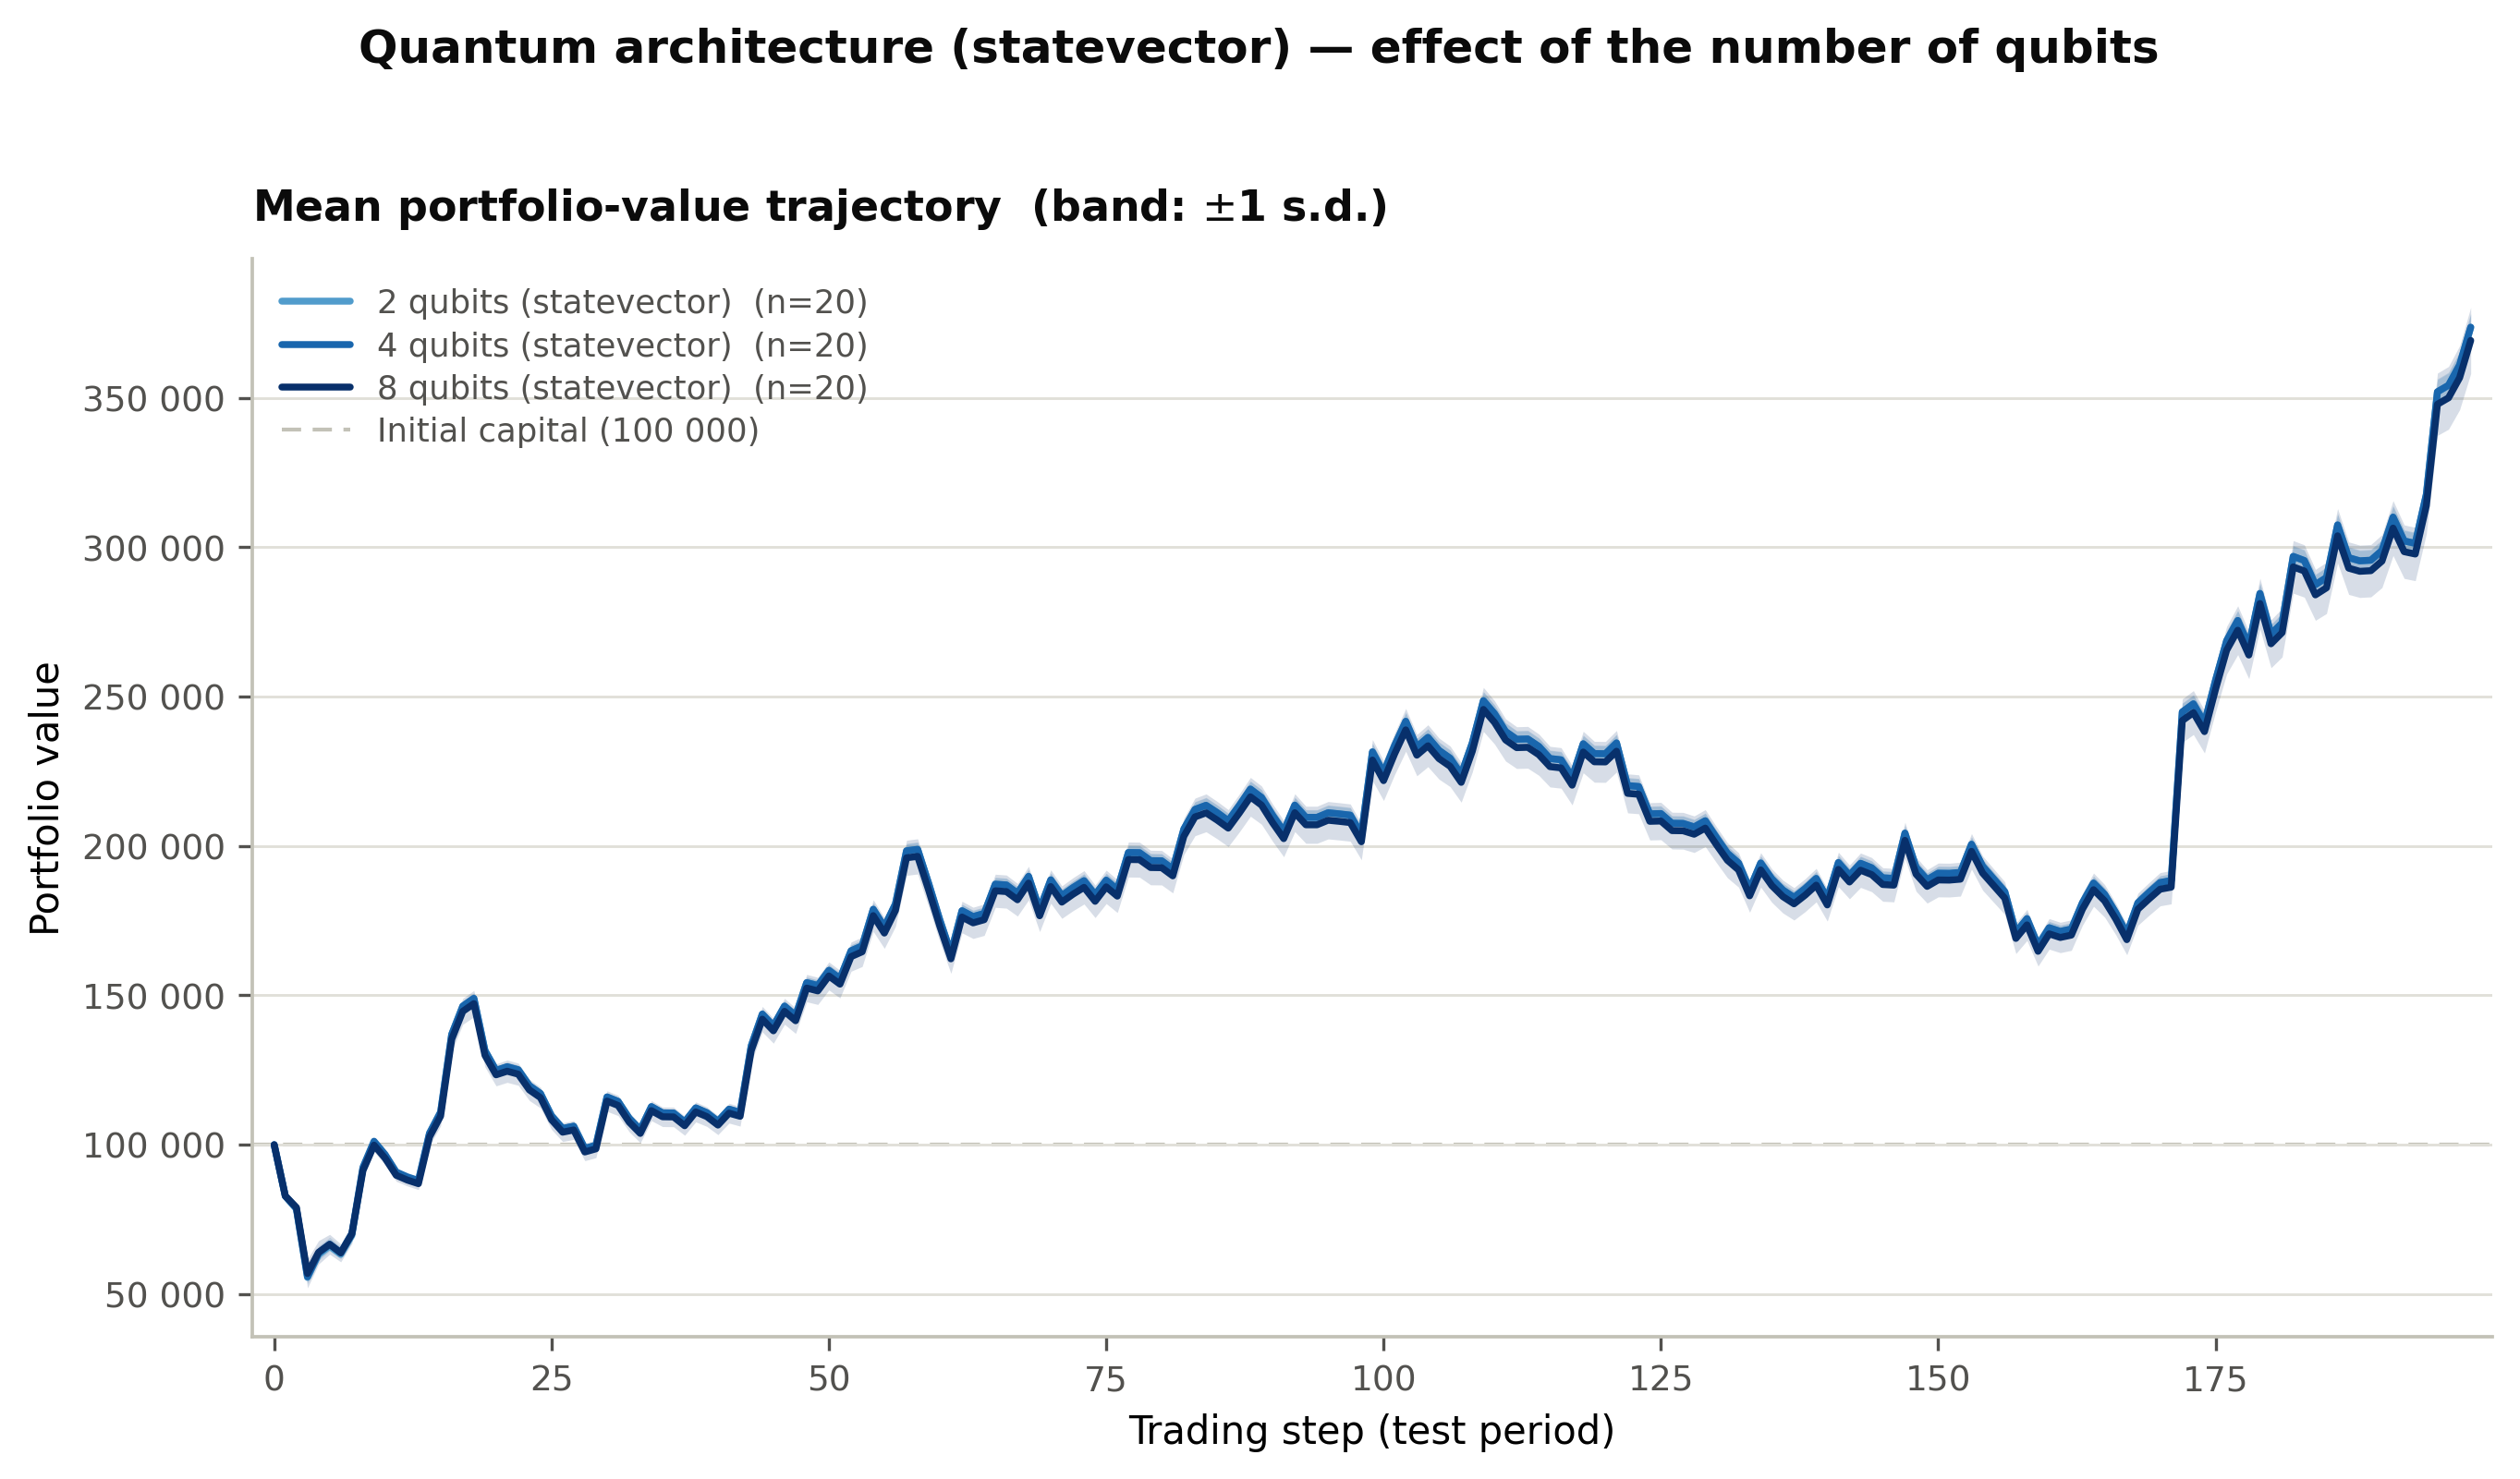
\includegraphics[width=\linewidth]{fig4_quantica_qubits.png}
  \caption{Quantum architecture under statevector simulation as a function of
  the width of the quantum latent layer: \num{2}, \num{4} and \num{8} qubits.
  Colour encodes the number of qubits on a single-hue scale, light to dark.
  Solid lines show the mean out-of-sample portfolio value and shaded envelopes
  denote $\pm 1$ standard deviation across $n = 20$ independent runs per
  configuration. The three
  widths are indistinguishable in final value (Kruskal--Wallis $H(2) = 2.13$,
  $p = 0.345$, $\varepsilon^2 = 0.002$), with mean final values of
  \num{373616}, \num{373668} and \num{369224} monetary units; the \num{8}-qubit
  configuration is the most dispersed of the three (standard deviation
  \num{11075} against \num{4327} and \num{4583}).}
  \label{fig:qubit-variation}
\end{figure}

\FloatBarrier
\subsection{Step 5 --- matched-width comparison}
\label{subsec:res-headtohead}

The two instantiations of the latent block can now be compared at the same
width, under the same protocol, inside the same network. At eight units, the
classical block reaches a mean final value of \num{301294} with a coefficient of
variation of \num{0.22}; the quantum block reaches \num{369224} with a
coefficient of variation of approximately \num{0.030}, using \num{16} trainable
parameters against \num{72}.

\ref{tab:summary} collects every campaign reported above on a common scale.
Read down the table, the ordering is consistent: the level rises and the
dispersion falls along the chain EI3 $\to$ scaffold $\to$ classical block $\to$
quantum block, and the largest single movement in dispersion occurs at the last
step.
\begin{table}[htbp]
  \centering
  \caption{Summary of all experimental campaigns. Each row reports the
  distribution of the final out-of-sample portfolio value (monetary units;
  initial capital \num{100000}) at the end of the 2020 test window, over
  $n$ independent training runs. s.d.\ is the sample standard deviation
  across runs and CV $= \mathrm{s.d.}/\text{mean}$ is the coefficient of
  variation, used as the scale-free measure of run-to-run dispersion.
  The first block characterises the EI3 baseline under three training
  configurations; all remaining rows use the unified protocol of
  table~\ref{tab:hyperparams} and differ only in the latent block:
  absent (scaffold), a dense $\tanh$ layer (72 parameters at 8 neurons),
  or a RealAmplitudes circuit with reps $=1$ and full entanglement
  ($2Q$ parameters) evaluated with exact expectation values. Quantum
  rows use the width-dependent seeds of eq.~\eqref{eq:seed}, so
  cross-model comparisons are between unpaired samples and are reported
  descriptively.}
  \label{tab:summary}
  \begin{tabular}{lccccc}
    \toprule
    Configuration & Latent block & $n$ & Mean & s.d. & CV \\
    \midrule
    EI3, reference impl.      & ---        & 20 & \num{192638} & \num{31608} & 0.164 \\
    EI3, 50 ep.\ / batch 8    & ---        & 20 & \num{216122} & \num{28132} & 0.130 \\
    EI3, 120 ep.\ / batch 200 & ---        & 20 & \num{224138} & \num{55409} & 0.247 \\
    \midrule
    QEI3-eq NoCL              & absent     & 20 & \num{280563} & \num{82410} & 0.294 \\
    QEI3-eq                   & 8 neurons  & 20 & \num{301294} & \num{65509} & 0.217 \\
    \midrule
    QEI3                      & 2 qubits   & 20 & \num{373616} & \num{4327}  & 0.012 \\
    QEI3                      & 4 qubits   & 20 & \num{373668} & \num{4583}  & 0.012 \\
    QEI3                      & 8 qubits   & 20 & \num{369224} & \num{11075} & 0.030 \\
    \bottomrule
  \end{tabular}
\end{table}

We deliberately refrain from declaring this difference significant. The
comparison is between batteries that were not seed-paired --- the classical
campaign ran under seed \num{42} and the eight-qubit quantum campaign under seed
\num{50}, per \ref{eq:seed-rule} --- and the corresponding hypothesis tests
have not yet been computed. What can be asserted at this stage is descriptive
and, we believe, still substantive: the quantum instantiation attains a higher
mean level with a dispersion roughly an order of magnitude smaller, and does so
at three distinct widths under three distinct seeds, whereas the classical
instantiation was not distinguishable from having no block at all under the same
sample size.

\begin{figure}[htbp]
  \centering
  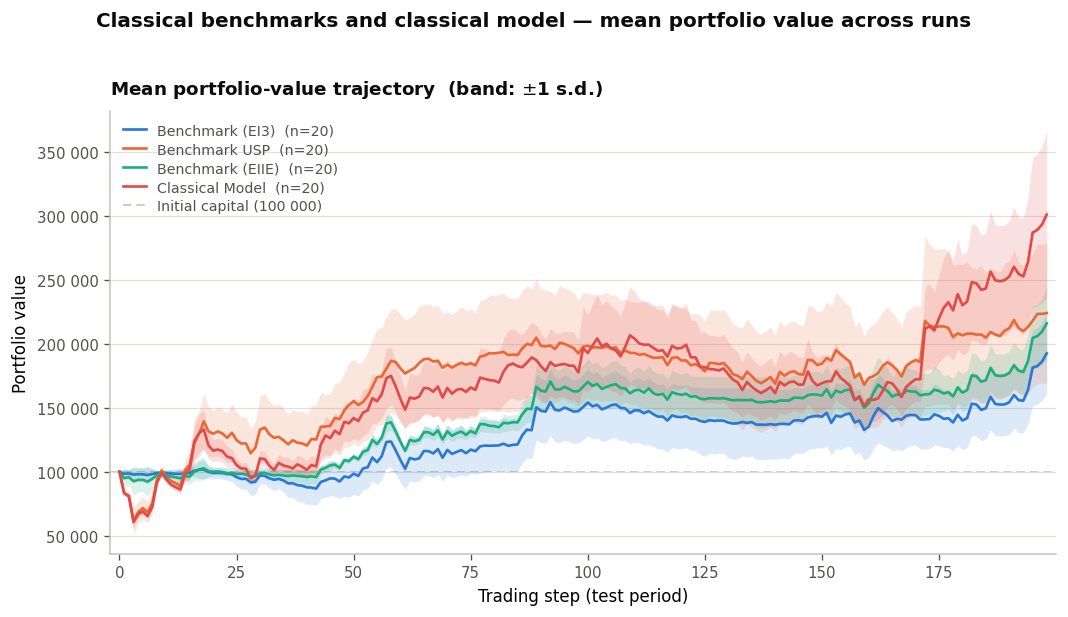
\includegraphics[width=\linewidth]{BenchmarkClassical.png}
  \todoitem{Decidir se tira }
  \caption{Mean out-of-sample portfolio value across independent runs for the
  classical baselines --- EI3, EIIE and the reference benchmark --- and the
  proposed classical model. Solid lines show the mean trajectory over the test
  period; shaded envelopes denote $\pm 1$ standard deviation across independent
  training runs per model. All agents start from the same initial capital of
  \num{100000} monetary units (dashed grey line) and are evaluated on an
  identical out-of-sample window.}
  \label{fig:benchmark-classical}
\end{figure}

% =====================================================================

% =====================================================================
% \bibliographystyle{splncs04}
\bibliography{ref}

https://arxiv.org/abs/2601.18811 % Paper extremamente relevante de QRL



\end{document}